\documentclass[11pt]{article}
% packages
\usepackage[utf8]{inputenc}
\usepackage[T1]{fontenc}
\usepackage{geometry}
\usepackage[pdftex]{graphicx}
\usepackage{graphicx}
\usepackage{tabularx}
\usepackage{dsfont}
\usepackage{multirow}
\usepackage{amsmath,amsfonts,amssymb}
\usepackage{subcaption}
\usepackage{authblk}
\usepackage{placeins}
\usepackage{epigraph}
%hyperlinks options
\usepackage{hyperref}
\hypersetup{colorlinks=true,linkcolor=blue,filecolor=magenta,urlcolor=cyan,citecolor=cyan}
%bib options
\usepackage[backend=biber,style=authoryear,bibstyle=authoryear,natbib=true,
giveninits=true,uniquename=false,uniquelist=false,% firstinits=false,
maxcitenames=2,date=year, maxbibnames=99,url=false]{biblatex}
\geometry{left=20mm, top=20mm, right=20mm}
%float barrier
\usepackage{placeins}
 \addbibresource{Thèse.bib}
\title{Chapitre 2 : Collecte et caractérisation des données de crues à Beaucaire}
\author{Mathieu}

\begin{document}
\maketitle


\tableofcontents

\section{Introduction}

\paragraph{} Le passé de Beaucaire, du XVII\textsuperscript{ème} au XIX\textsuperscript{ème} siècle était indéniablement tourné vers le commerce fluvial. La foire de Beaucaire, d'importance européenne, attirait alors des marchands venus des quatre coins de la Méditerranée (figure \ref{fig:foire}). La ville de Beaucaire était considérée comme "\textit{la capitale française des marchandises}" \citep{leon_vie_1953} grâce à sa proximité avec la mer et les échanges fluviaux rendus possibles par son port sur le Rhône. L'attention des Beaucairois était alors tournée continuellement vers le fleuve et ses caprices, aussi bien sur les crues que sur les étiages fréquents qui perturbaient le commerce fluvial, source principale des revenus Beaucairois avant l'avènement du chemin de fer. A cette époque, Beaucaire et Tarascon étaient reliées par un pont de bateaux, qui, jusqu'à la construction d'un pont en pierre en 1830, servait à passer d'une ville à l'autre. Ce pont était régulièrement détruit par les crues, comme en en 1745 : "\textit{le pont de bateaux de Tarascon alla heurter et emporter celui d'Arles}" \citep{anibert_annales_1764}. Du fait de cet intérêt majeur pour le fleuve, le Rhône à Beaucaire fut l'une des premières stations limnimétriques françaises avec des relevés continus dès le début du XIX\textsuperscript{ème} siècle. + souligner la construction du canal de Beaucaire à la mer + dates construction

\begin{figure}[h]
		\centering
            \begin{subfigure}{0.49\linewidth}
            \centering
            	\includegraphics[width=1\linewidth]{Figures/foire4.jpg}\hfill
            	\caption{}
            	\label{subfig:foire1}
            \end{subfigure}
            \begin{subfigure}{0.49\linewidth}
            \centering
            	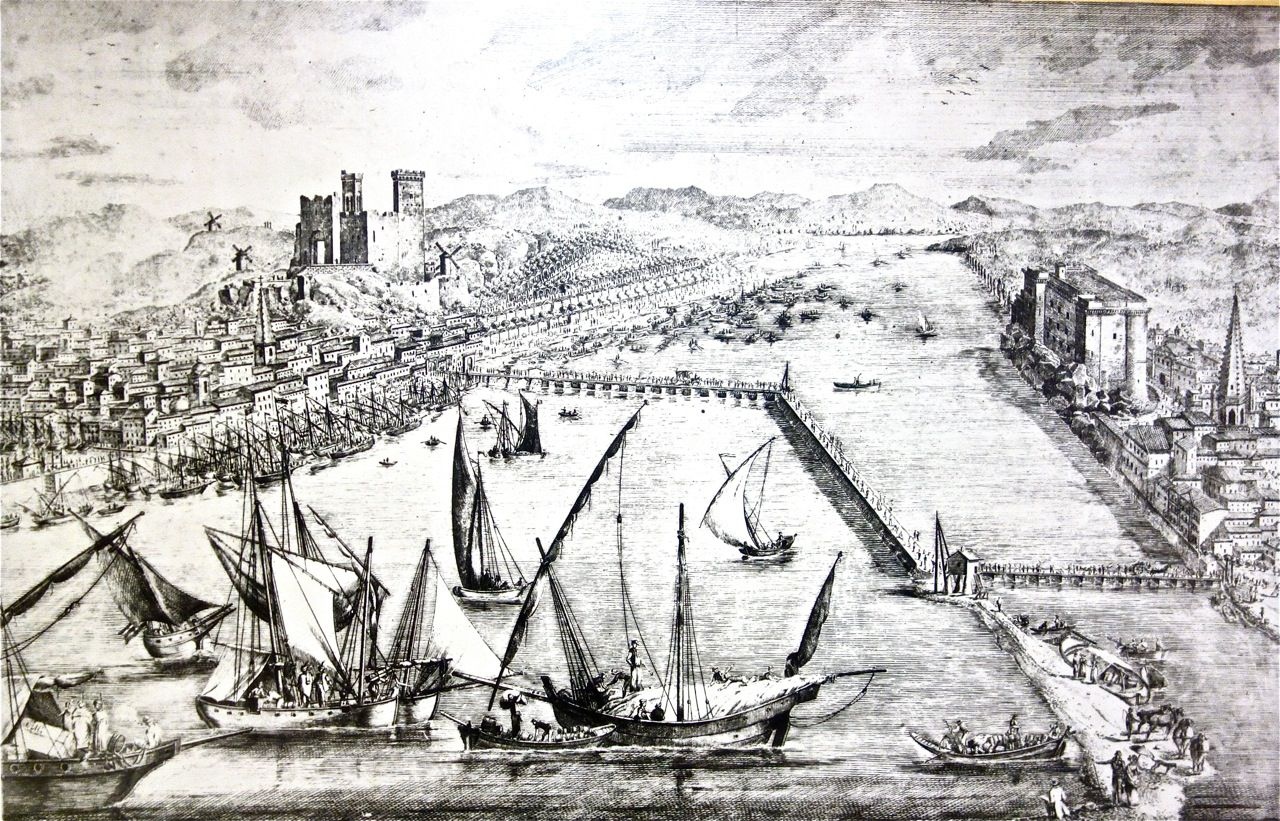
\includegraphics[width=1\linewidth]{Figures/foire5.jpg}
            	\caption{}
           		\label{subfig:foire2}
            \end{subfigure}
\caption{(a) "\textit{Vue de la foire de Beaucaire avec une partie de la ville de Tarascon}", Basset André (1749). On distingue la ville de Beaucaire sur la droite et Tarascon sur l'autre rive. 
(b) Pont de bateaux reliant Beaucaire à Tarascon lors de la foire, auteur inconnu (XVIII\textsuperscript{ème} siècle). Le pont était alors régulièrement détruit lors des crues, empêchant toute communication entre les deux villes.}
\label{fig:foire}
\end{figure}

\section{Hydrométrie du Rhône à Beaucaire de 1816 à aujourd'hui}

	\subsection{Contexte hydrologique et hydrométrique}
	
	\paragraph{} Le Rhône à Beaucaire draine un bassin versant de 95 590 km² et son module est de 1680 m\textsuperscript{3}/s (1920-2023) (REF MEDD). Beaucaire est la station hydrométrique la plus à l'aval du Rhône "complet", située 5 km à l'aval la confluence avec le Gardon (le dernier affluent du Rhône) et 10 km à l'amont de la diffluence qui donne naissance au Petit-Rhône et au Grand-Rhône (figure \ref{fig:BV}). Il s'agit donc de la station mesurant le débit le plus important du fleuve, mais également de France, le Rhône étant le premier fleuve français en terme de débit (à l'exception du Rhin qui est frontalier). Au delà de son important débit, le Rhône est un fleuve complexe de par la diversité de ses apports, comme décrit par \citet{parde_regime_1925} : "\textit{Dans une infinité de nuances et de contrastes, la Massa, l'Arve, l'Isère, la Durance, l'Ain, la Saône, l'Ardèche, c'est-à-dire des cours d'eau appartenant à toutes les catégories qu'on puisse trouver en Europe occidentale. [...] Ainsi, c'est par une carrière agitée que le petit torrent glaciaire de Gletsch devient le fleuve majestueux de Beaucaire, tour à tour ou en même temps nival et séquanien, océanique et méditerranéen, pondéré ou sujet aux plus déconcertants accès de démence}". A Beaucaire, les signatures des affluents alpins, océaniques, méditerranées et cévenols se mélangent pour donner naissance à un régime hydrologique qu'il est difficile de classer dans une catégorie (figure \ref{fig:Regime}). Il en est de même pour ses crues, qui sont le reflet de la complexité de ses apports : "\textit{Il est violent par son courant encore inapaisé tout près de la Méditerranée, par ses crues de plus en plus nombreuses, désordonnées et massives, à mesure qu'il approche du terme de son cours}" \citep{parde_regime_1925}. 


DESCRIPTION INSTRUMENTATION EN 2 STATIONS ET HISTORIQUE BCR

	\begin{figure}[h]
	\centering
		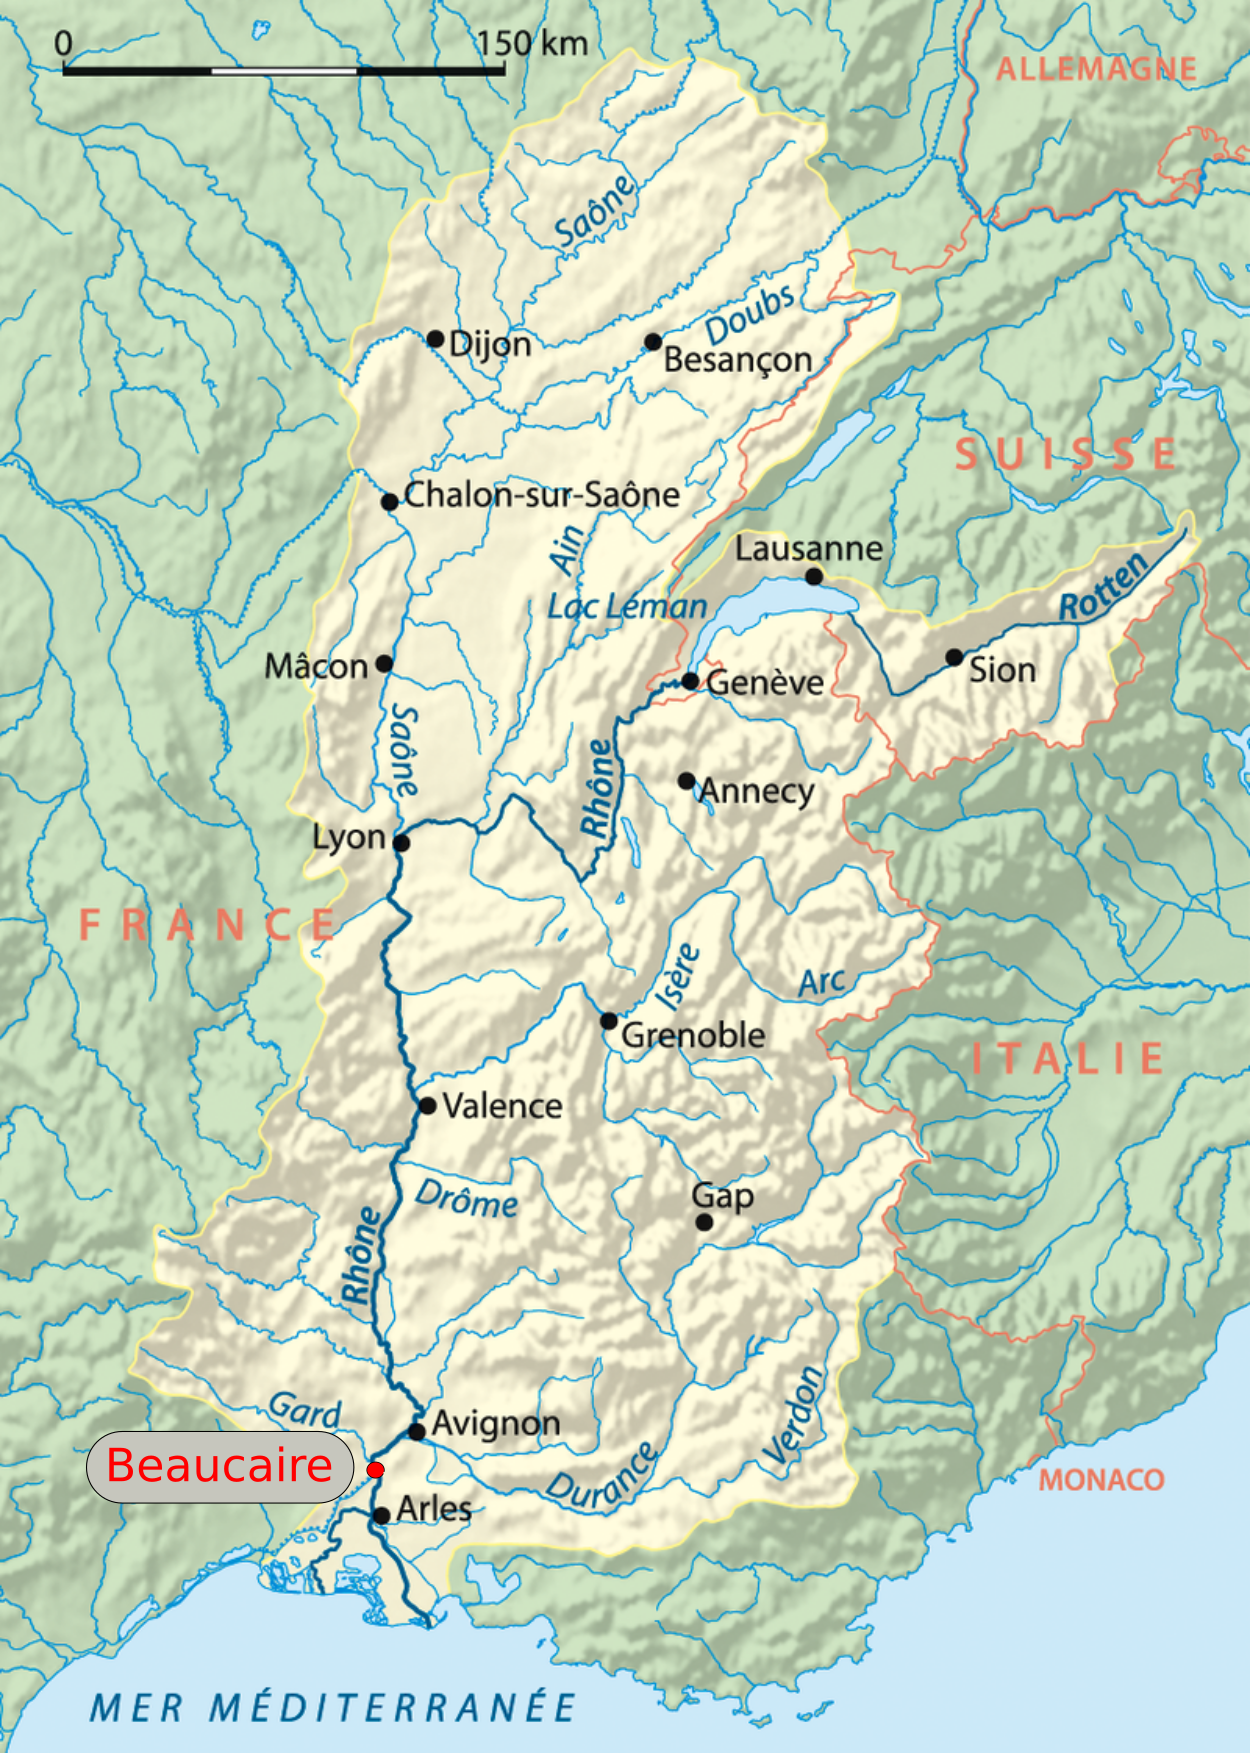
\includegraphics[width=.5\linewidth]{Figures/Rhone_bassin_versant.png}
        \caption{Bassin versant du Rhône. La ville de Beaucaire est indiquée en rouge (www.openstreetmap.org)}	
		\label{fig:BV}
	\end{figure}
	
	\begin{figure}[h]
	\centering
		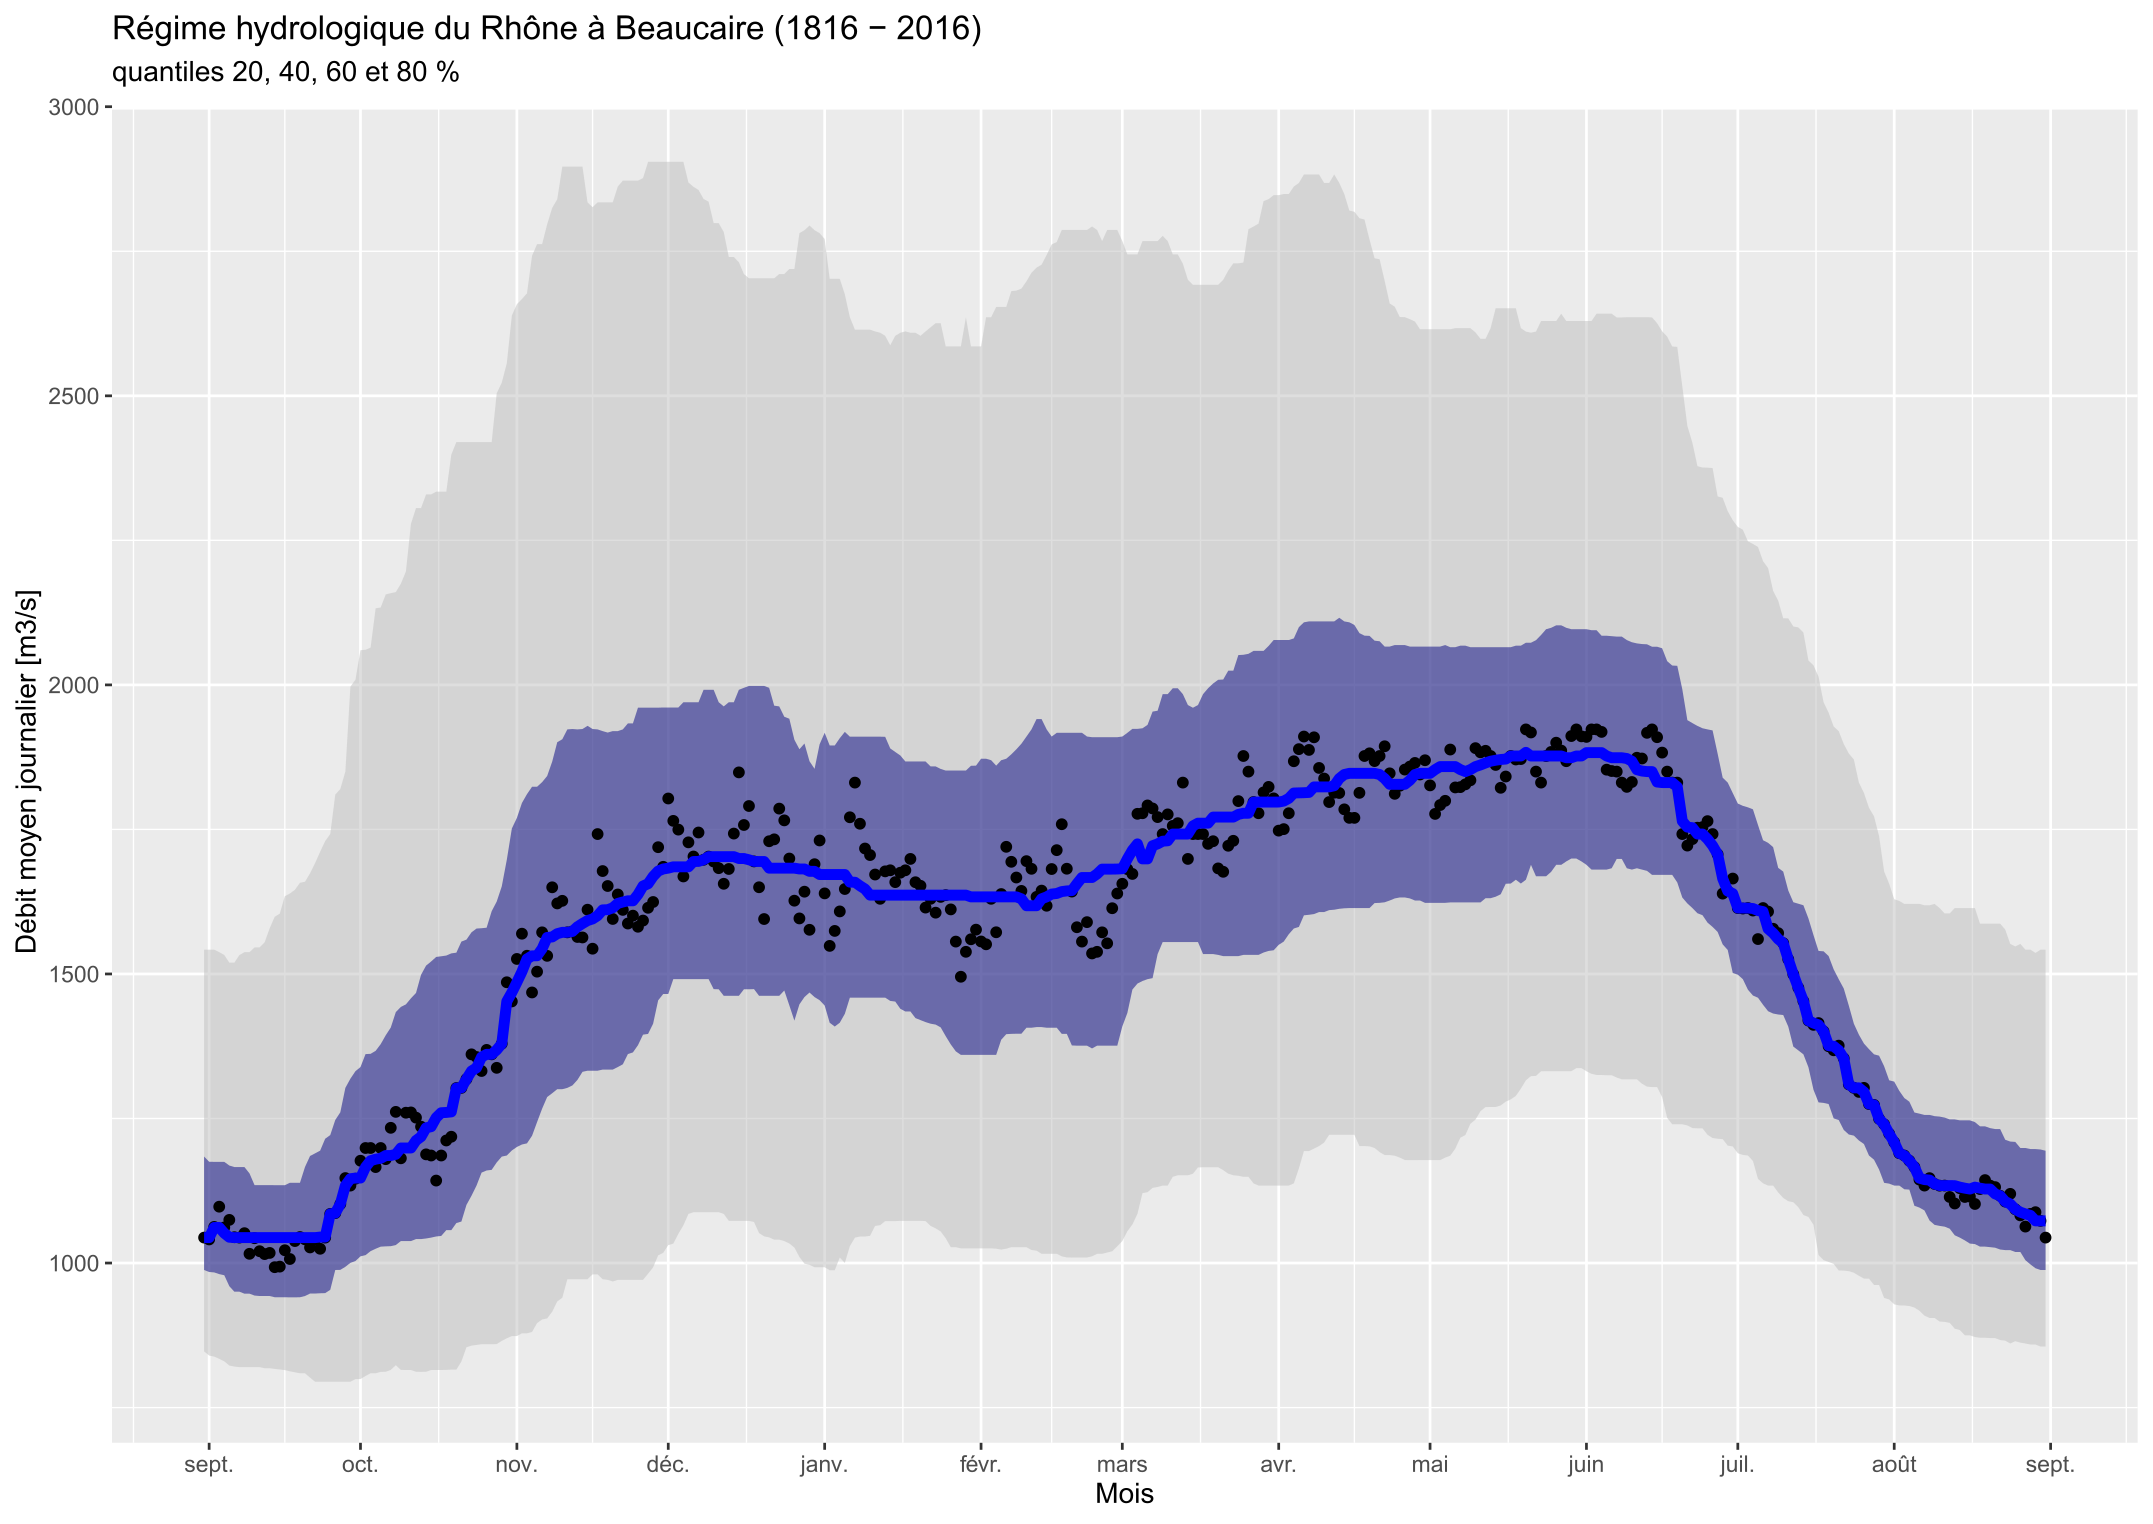
\includegraphics[width=.7\linewidth]{Figures/RegimeModif.png}
        \caption{Débit moyen journalier du Rhône à Beaucaire (1816-2016). En bleu foncé, les quantiles 40 et 60\%, en gris les quantiles 60 et 80\%.}	
		\label{fig:Regime}
	\end{figure}
	
	
\FloatBarrier

	\subsection{Station hydrométrique du Rhône à Pont de Beaucaire (1816-1967)}
	
	\paragraph{} Le travail d'archives de \citet{pichard_les_1995} et \citet{pichard_hydro-climatology_2017} a permis de reconstituer une chronique continue d'observations de la hauteur d'eau du Rhône à Beaucaire à partir du 15 Mai 1816 (tableau \ref{tab:MesuresPtBcr}). Ces relevés semble être les plus anciens qu'il soit possible de retrouver à Beaucaire (\citet{pichard_les_1995}; \citet{parde_regime_1925}). L'échelle limnimétrique fut installée sur le musoir de l'écluse du canal de Beaucaire à la mer (au point kilométrique 267.7), dont les travaux furent achevés en 1811. \citet{pichard_hauteurs_2013} souligne que "\textit{la longévité et la stabilité de cette échelle est évidemment exceptionnelle pour le bas Rhône. [...] La documentation chiffrée y est aussi précieuse et abondante qu'à Arles, mais cependant toujours aussi dispersée et accessible la plupart du temps par copie et non par les feuilles d'observations originales que les organismes gérants n'ont pas su conserver, en raison de transferts permanents d'attributions}". Il faut noter que l'écluse du canal de Beaucaire fut remplacée entre 1914 et 1918 par une autre écluse débouchant plus à l'aval. Il semble cependant que le musoir que l'on observe de nous jours existait dès l'origine du canal et que l'échelle n'a subi aucun déplacement (\citet{pichard_hauteurs_2013}; \citet{bard_actualisation_2018}). 
	
	\begin{figure}[h]
	\centering
		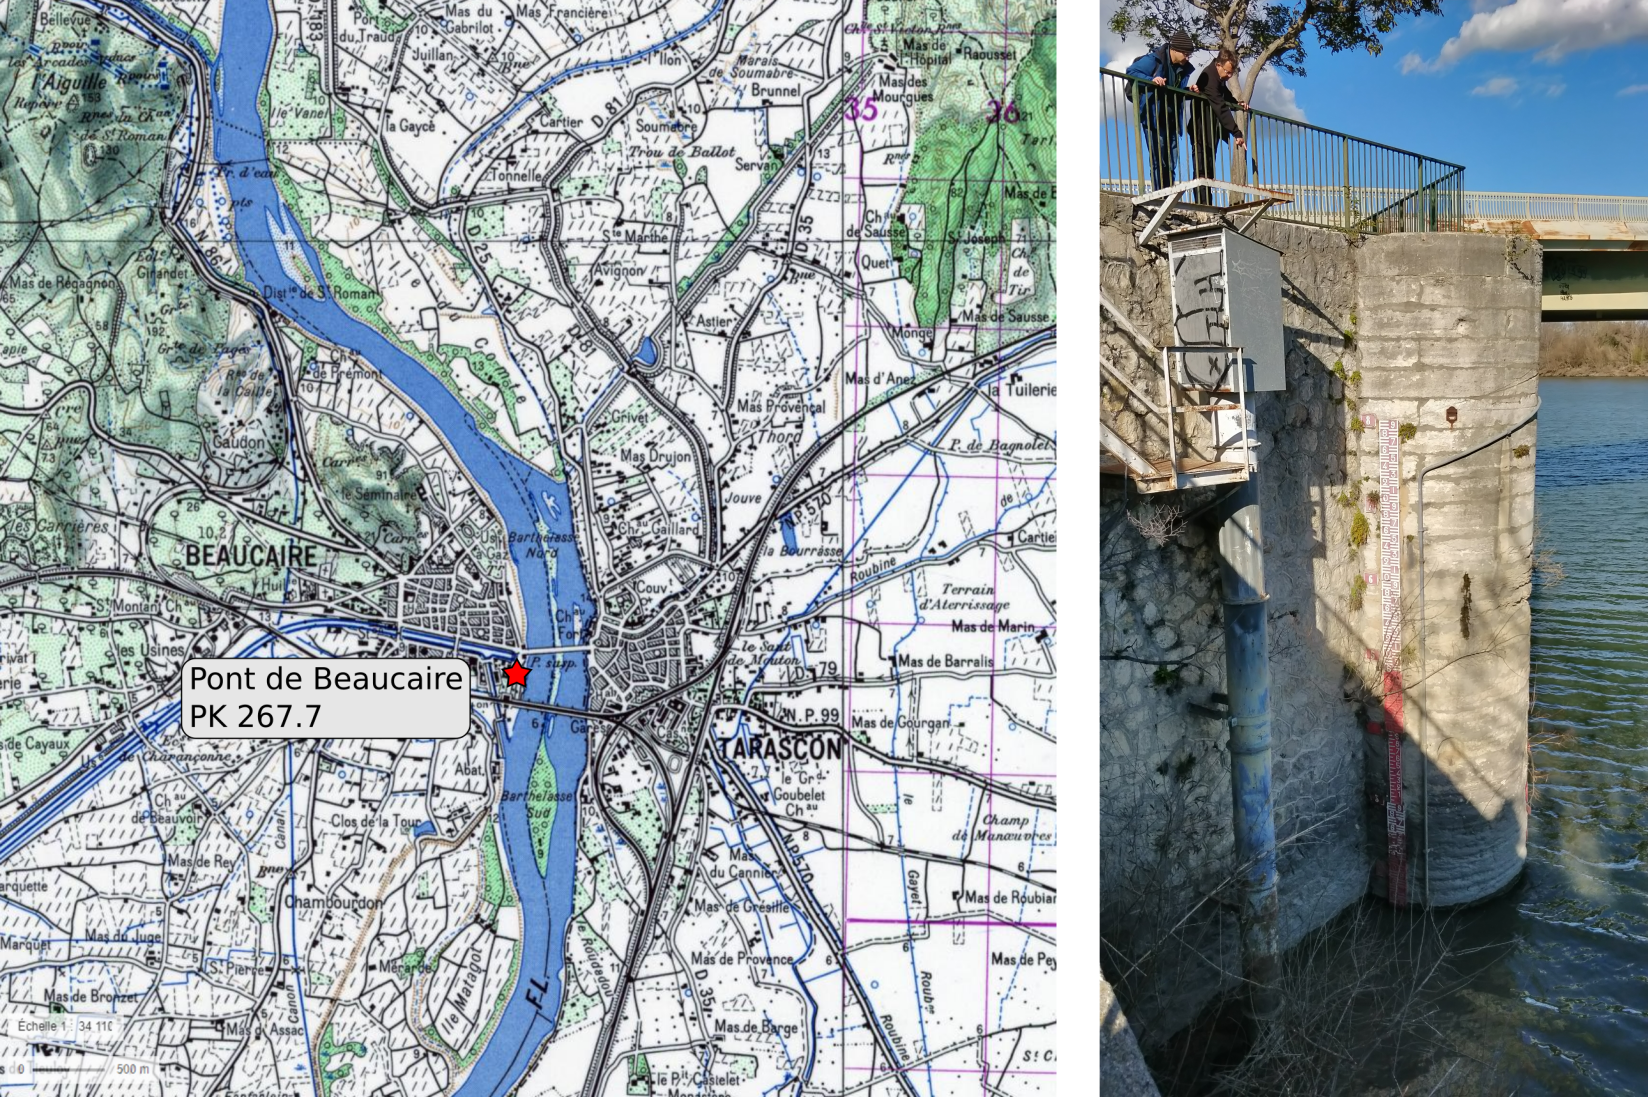
\includegraphics[width=.7\linewidth]{Figures/PtCartoPhoto.png}
        \caption{(Gauche) Localisation de la station de Pont de Beaucaire (carte IGN 1950, source : www.geoportail.fr). (Droite) Échelle et limnigraphe CNR de Pont de Beaucaire en Février 2020.}	
		\label{fig:CartoPt}
	\end{figure}
		
	\subsubsection{Relevés disponibles}
	\paragraph{} Les relevés retrouvés correspondaient probablement à une lecture d'échelle quotidienne en milieu de journée. Après la crue généralisée de 1840 et la création du Service Spécial du Rhône, une norme de trois relevés par jour (à 7h, 12h et 17h) se met lentement en place (figure \ref{fig:RelevesPt}). L'application de cette norme n'est visible dans les données qu'à partir de 1887, et ce jusqu'à la fin de l'exploitation de la station.  L'année 1967 marque le début des travaux d'aménagement de l'ouvrage hydroélectrique de Vallabrègues et de son canal de dérivation réalisés par la Compagnie Nationale du Rhône (CNR). Cette dérivation étant restituée à l'aval de la ville de Beaucaire, la station est déplacée 2 km plus à l'aval, environ 600 m à l'aval de la restitution des débits transitant par la centrale hydroélectrique. La nouvelle station, exploitée par la CNR à partir de 1970, sera alors appelée "Beaucaire Restitution".
	
	\begin{figure}[h]
          \centering
            \begin{subfigure}{0.49\linewidth}
            \centering
            	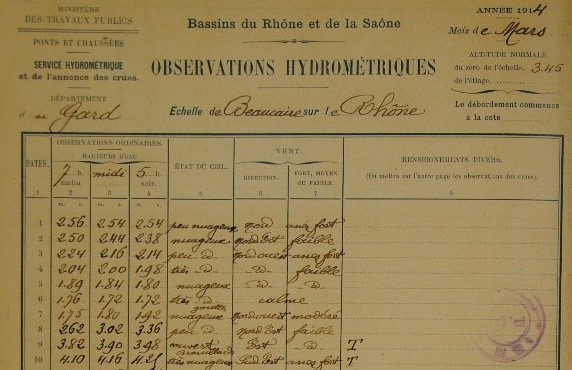
\includegraphics[width=1\linewidth]{Figures/TabObsBcrSmall.jpg}\hfill
            	\caption{}
            	\label{subfig:TabObsPt}
            \end{subfigure}
            \begin{subfigure}{0.49\linewidth}
            \centering
            	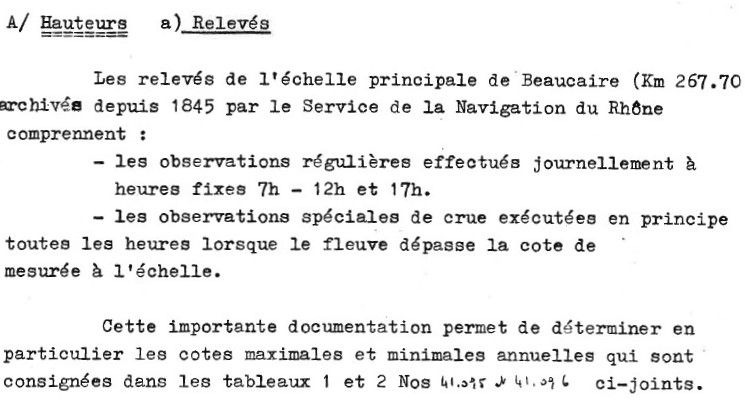
\includegraphics[width=1\linewidth]{Figures/RegleStationCNR}
            	\caption{}
           		\label{subfig:RegleCNR}
            \end{subfigure}
      \caption{(a) Feuille originale des relevés de hauteur d'eau à Beaucaire réalisés par le service spécial du Rhône en Mars 1914. On remarque les trois relevés par jour ainsi que des précisions sur l'état du ciel ou le vent. (b) Règles d'exploitation de la station de Pont de Beaucaire, fiche station de la CNR. On remarque que des observations horaires sont effectuées en crue mais la cote est effacée sur ce document (Source : Archives CNR, 1962)}
	 \label{fig:RelevesPt}
		
	\end{figure}            
            
    
	\begin{table}[h]
	\centering
	\caption{Détail des données de la station de Pont de Beaucaire (PK 267.7)}
    \label{tab:MesuresPtBcr}
	\resizebox{\columnwidth}{!}{%  
       \begin{tabular}{|c|c|c|c|c|c|} 
                \hline
               Période & Périodicité & Méthode & Origine & Zéro échelle & Commentaire \\
                \hline
                1816-1886 & 1 mesure/jour & Visuelle & 
                Service Spécial du Rhône & 3.34 mNGFo & Probablement mesure à 12h \\
                \hline
                1887-1967 & 3 mesure/jour & Visuelle & 
                Service Spécial du Rhône & 3.34 mNGFo & Relevés à 7h, 12h, 17h\\
                \hline
               1970-2020 & Horaire & Limnigraphe à flotteur puis LPN8 & 
                BD CNR & 0.03 mNGFo &  \\
                \hline
		\end{tabular}
		}
        \end{table}           
        
       
    \paragraph{} Les jaugeages les plus anciens récupérés dans les archives départementales du Rhône datent de 1845 (figure \ref{fig:Jau1845}) alors que les mesures limnimétriques débutent en 1816. Il faut noter que tous les jaugeages ont été effectués à l'amont de Beaucaire dans une zone plus stable et dépourvue d'îles (excepté les quatre jaugeages de 1845 et 1846, effectués au droit de la station de Pont de Beaucaire). Un total de 233 jaugeages est disponible à Pont de Beaucaire, couvrant la période 1845-1967, avec une fréquence peu homogène et des périodes non-jaugées (en période de guerre par exemple). 
    
    \begin{figure}[h]
	\centering
		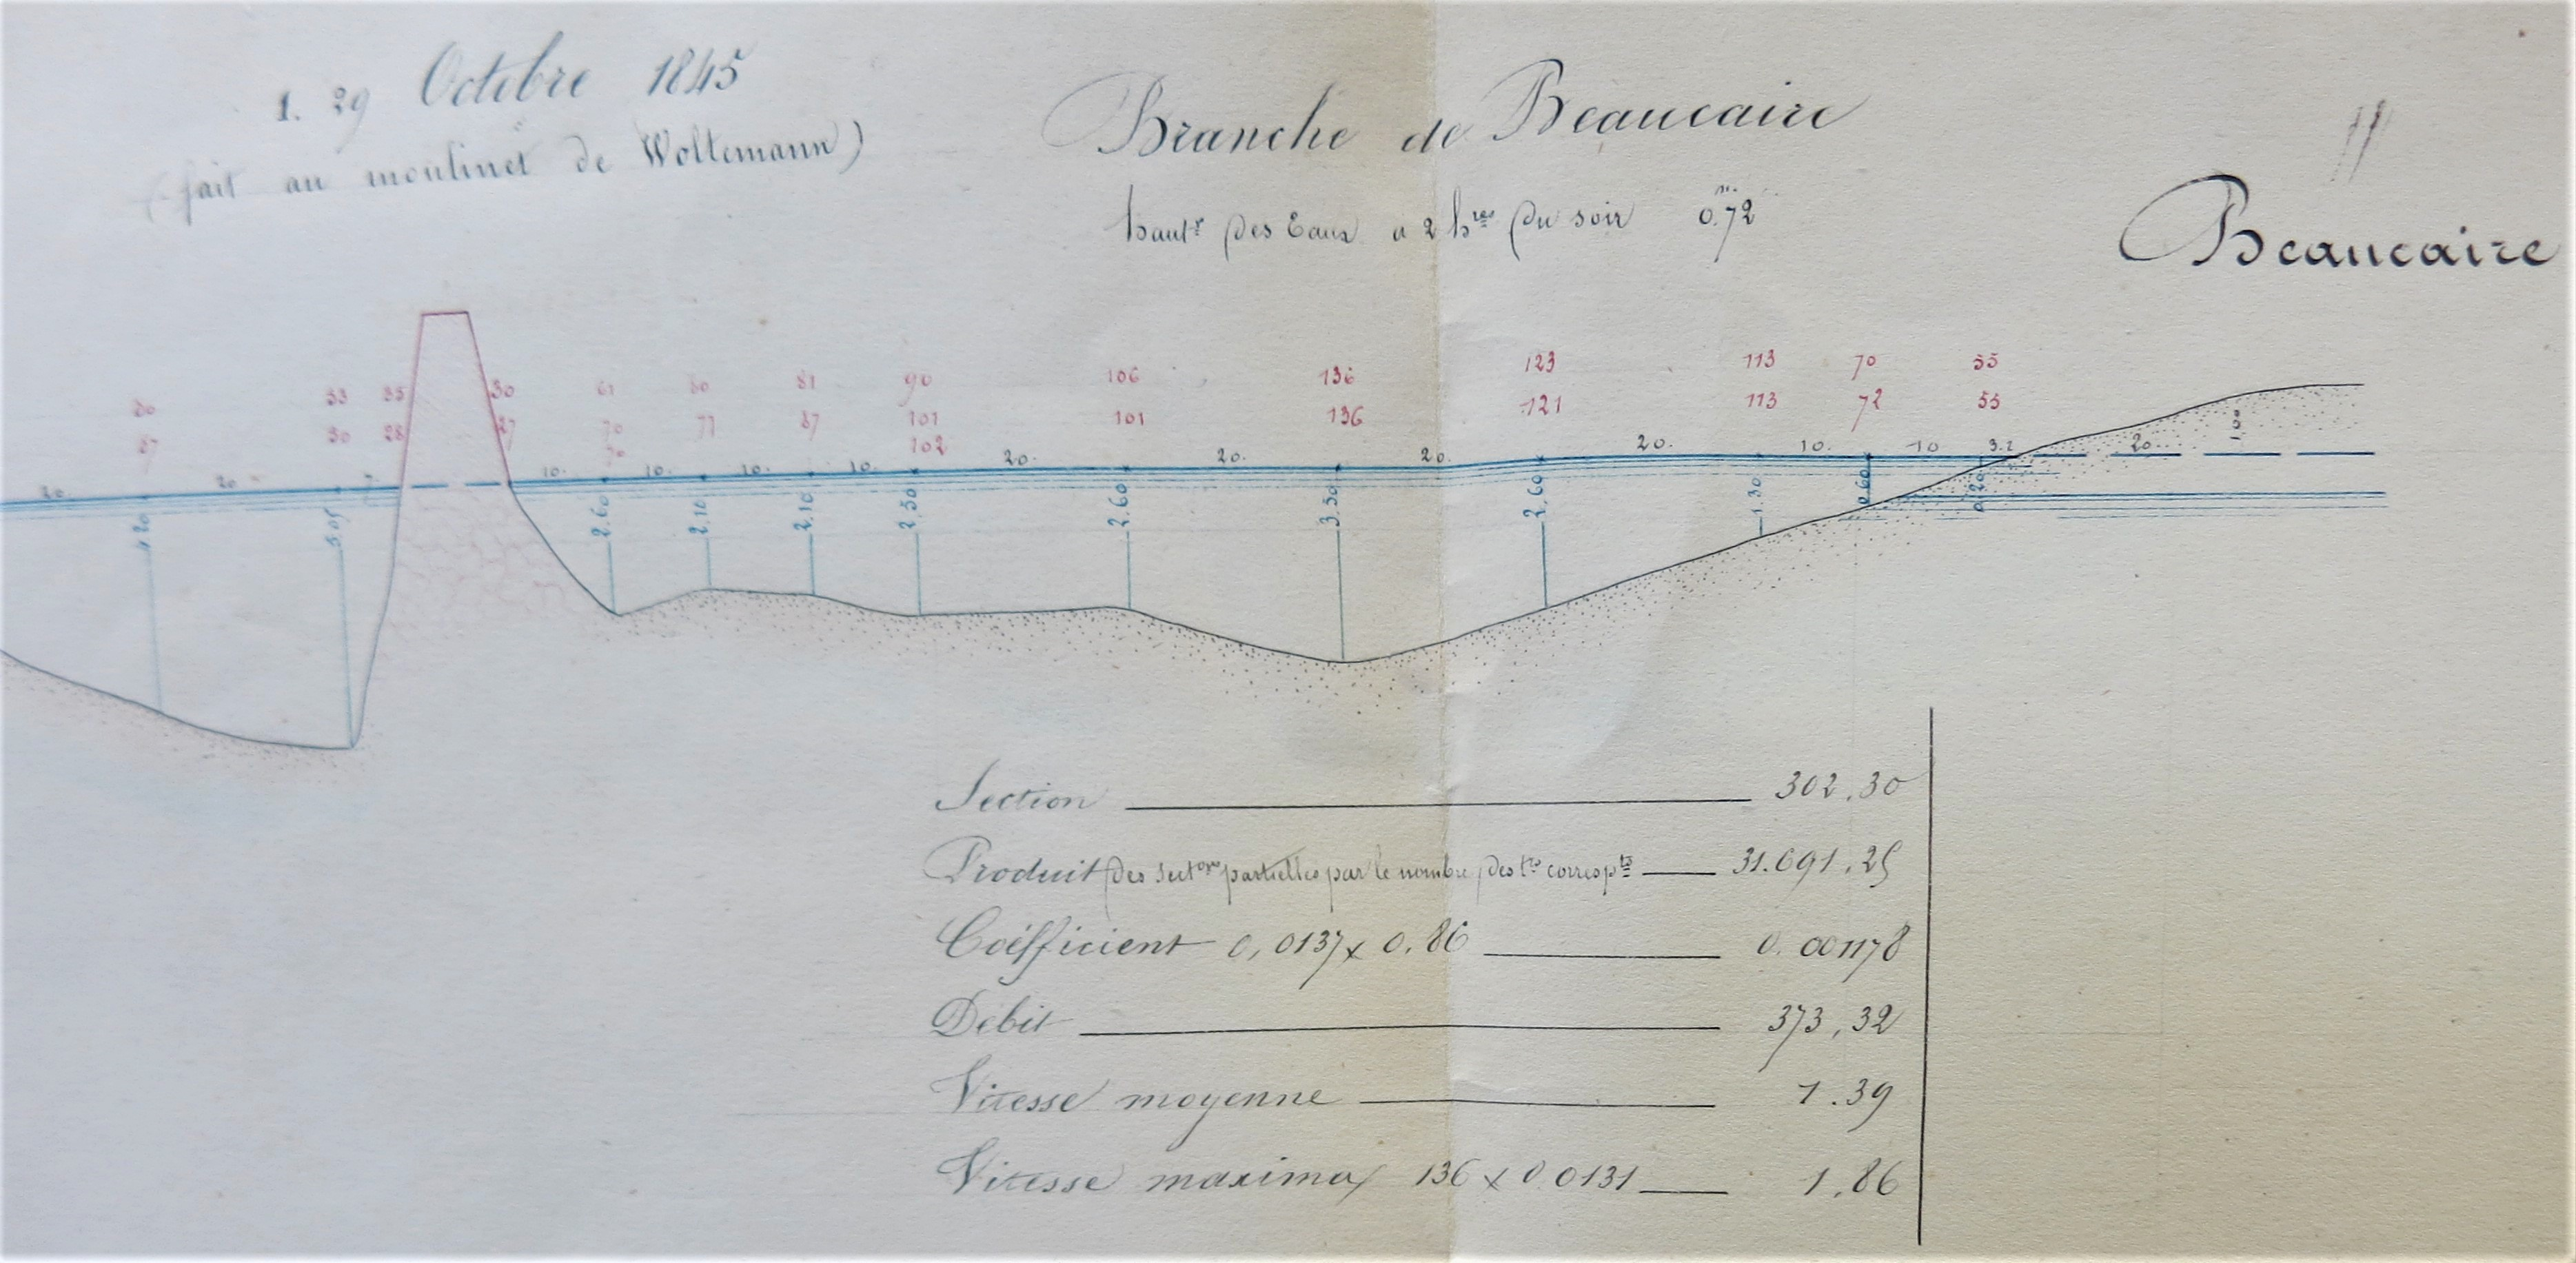
\includegraphics[width=.7\linewidth]{Figures/Jau1845.jpg}
        \caption{Jaugeage du 29 Octobre 1845 au droit de la station de Pont de Beaucaire, réalisé au moulinet de Woltmann par le Service Spécial du Rhône. En bas à droite, le détail du calcul du débit. Les chiffres en rouge représentent le nombre de tours du moulinet, probablement moyennés sur une verticale.}	
		\label{fig:Jau1845}
	\end{figure}
    
    Plot de l'ensemble des jaugeages disponibles?
	
	\subsubsection{Évolution de l'altitude du zéro de l'échelle}
    
    \paragraph{} Comme attesté par \citep{pichard_hauteurs_2013}, l'échelle limnimétrique de Pont de Beaucaire possède le rare avantage d'être restée à la même place depuis 1816, avec une altitude du zéro relativement stable dans l'histoire. Malgré les divers changements de référentiels altimétriques durant l'histoire, le zéro semble n'avoir que très peu varié (Tableau \ref{tab:zeroPt}). De la même manière que \citet{bard_actualisation_2018}, nous retiendrons la dernière mesure de la CNR qui semble être une valeur médiane de l'ensemble des valeurs connues : 3.37 m NGF IGN69 / 3.34 m NGF ortho (ou Lallemand). De plus, celle-ci est compatible avec les valeurs données lorsque la station était encore exploitée.

            \begin{table}[h]
                \centering
                \caption{Mesures de l'altitude du zéro de l'échelle à Pont de Beaucaire}
            	\label{tab:zeroPt}
                \begin{tabular}{| m{3cm} | m{3cm}| m{3cm} | m{3cm} |} 
                    \hline
                    Date & Altitude du zéro en m NGF IGN69 & Altitude du zéro en m NGFortho	& Organisme \\
                    \hline
                    1959 &	3.375 &	3.345 &	CNR\\
                    \hline
                    1961 &	3.36 &	3.33 &	CNR\\
                    \hline
                    2010 &	3.38 &	3.35 &	Symadrem\\
                    \hline
                    2010 &	3.37 &	3.34 &	CNR\\
                    \hline
            \end{tabular}
        \end{table}


\FloatBarrier
		\subsubsection{Travaux et aménagements}
    	\label{subsubsec:TravauxPt}
    
    \paragraph{} La largeur de la section du Rhône au niveau de Beaucaire (ou du moins, la largeur du lit majeur) n'a que peu évolué dans l'histoire car elle se situe au niveau d'un resserrement entre deux collines rocheuses. Ce resserrement est bien visible sur les champs d'inondation de 1840 et 1856 (Figure \ref{Champ1856}). En revanche, à une échelle plus réduite, de nombreuses modifications morphologiques, d'origine naturelle ou anthropiques ont pu affecter l'écoulement et modifier la relation hauteur/débit durant les deux siècles de relevés limnimétriques. Ces modifications sont listées dans les paragraphes suivants.
    
    \begin{figure}[h]
        \centering
        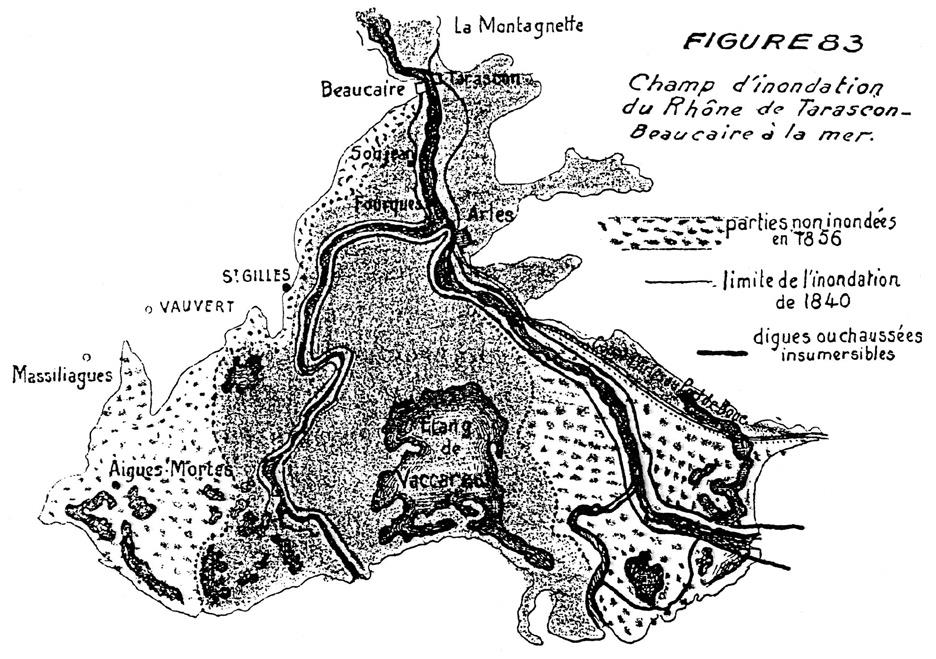
\includegraphics[width=.6\linewidth]{Figures/ChampInond1840-1856.jpg}
        \caption{Champ d'inondation du Rhône aval des crues de 1840 ou 1856, d'après \citet{parde_regime_1925}}
        \label{Champ1856}
    \end{figure}
    

	\paragraph{} Le premier pont reliant Beaucaire à Tarascon date de 1829. Il s'agit d'un pont suspendu composé de 4 piles (d'après la carte d'état-major de 1840), situé environ 30 m à l'amont du pont actuel, soit environ 45m à l'amont de l'échelle limnimétrique. Quelques années plus tard, en Juillet 1852, était inauguré le viaduc de chemin de fer de Beaucaire. Il est situé environ 250 m à l'aval de la station. Par la suite, les seuls travaux qui ont eu lieu dans le secteur sont ceux de l'aménagement CNR de Vallabrègues, entre 1967 et 1970. Ils ont sonné la fin de l'utilisation de la station par la CNR, devenue non-significative de la totalité du débit du Rhône suite à la création du canal de dérivation de l'aménagement. On peut noter la construction du pont routier actuel, entre 1988 et 1990, 30 m à l'amont de l'ancien pont. 
        

        \paragraph{} Depuis l'époque des plus anciennes cartes et récits retrouvés à Beaucaire jusqu'à aujourd'hui, des bancs de sable et îlots de diverses formes et dimensions ont séparé l'écoulement en deux bras plus ou moins distincts selon les périodes. De tout temps, mais pour des hauteurs d'eau différentes, les deux bras ont communiqué, un bras prenant le dessus sur l'autre au gré des événements morphogènes. Petit à petit, ces îlots ont été fixés par des digues afin de faciliter la navigation dans la zone, pour finalement arriver à la situation actuelle de deux bras bien distincts (figure \ref{fig:CartoRes}), comme en témoigne la carte d'\citet{armand_ii_1907} (figure \ref{fig:DigArmand}) qui décrit les différentes étapes de cette séparation. 
        
         \begin{figure}[h]
            \centering
            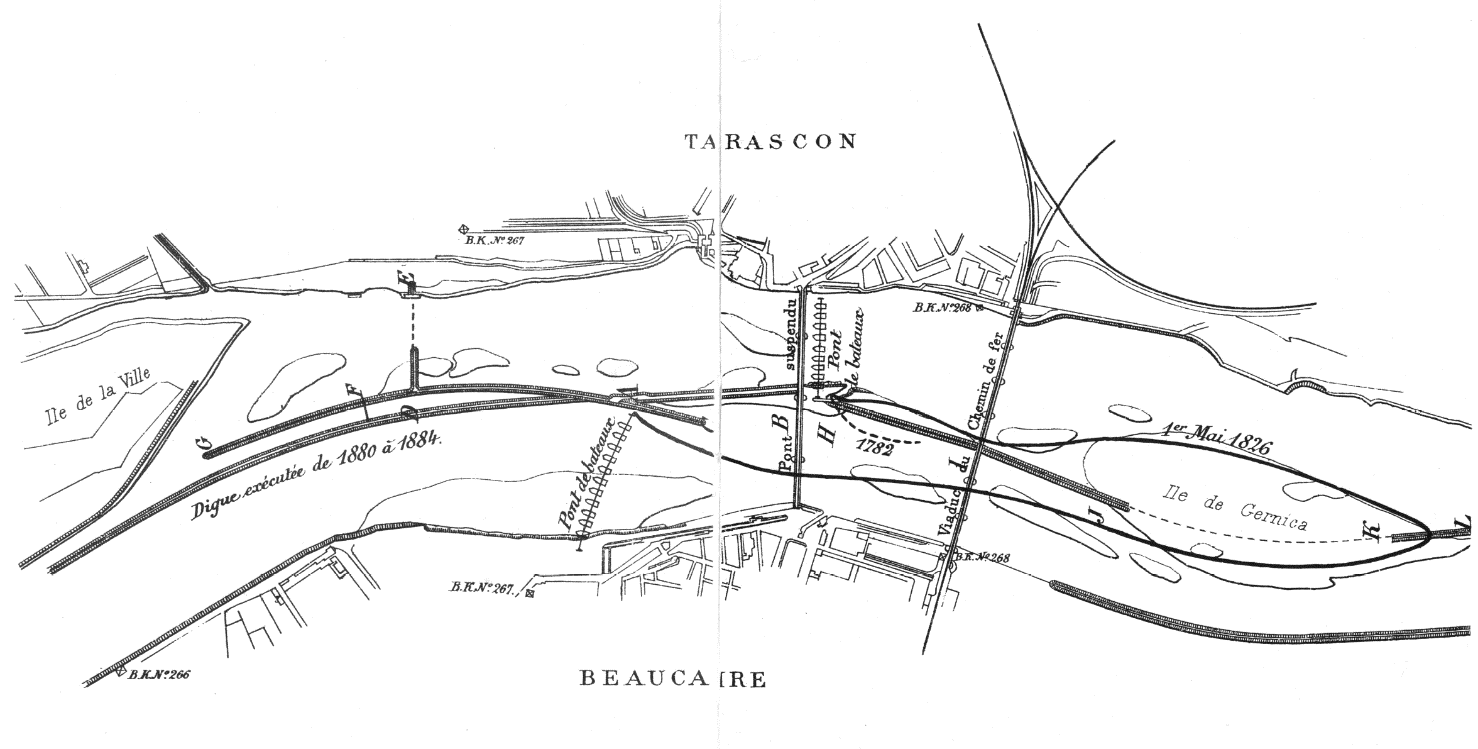
\includegraphics[width = 0.8\linewidth]{Figures/DiguesArmand.png}
            \caption{Carte de l'historique des digues de Beaucaire \citep{armand_ii_1907}}
            \label{fig:DigArmand}
        \end{figure}
        
        \begin{itemize}
            \item[$\bullet$] Digue divisoire (\textbf{AB}), antérieure à 1782
            \item[$\bullet$] Atterrissement (trait plein noir sur la carte) qui, dès 1826 se prolongeait jusqu'au point aval de l'île de Gernica. Il était probablement déjà présent au début du 19ème siècle.
            \item[$\bullet$] Érosion de l'île de la ville (à l'amont de Beaucaire) qui a modifié la répartition des débits entre les deux bras en faveur du bras de Tarascon. Pour maintenir la navigation dans le bras de Beaucaire, la digue \textbf{AB} fut prolongée à l'amont par une digue concave \textbf{CDF} en 1851 et par la suite, obstruction partielle du bras de Tarascon entre 1852 et 1855 \textbf{DE}. On peut constater cette érosion très rapide en faveur du bras de Tarascon sur les profils en travers de Goux (1850) (Figure \ref{fig:ProfGoux}). L'érosion de l'île de la ville peut être attribuée notamment à la crue catastrophique de 1840, possible déclencheur de ce phénomène.
            \item[$\bullet$] Forte érosion de l'atterrissement au niveau de \textbf{HI} du fait de l'écart de hauteur d'eau entre les deux bras pendant les crues. Une digue fut construite entre 1858 et 1859 pour pallier à ce phénomène.
            \item[$\bullet$] Pour ces mêmes raisons, construction d'une digue en aval du viaduc de chemin de fer \textbf{IJ} en 1872-1875 ainsi que la digue \textbf{KL} à l'aval de l'île de Gernica, qui se prolonge actuellement sur 2km vers l'aval.
            \item[$\bullet$] Prolongement de la digue concave \textbf{GF} autour de 1875
            \item[$\bullet$] Construction d'une nouvelle digue concave à l'amont de \textbf{GF} entre 1880 et 1884
        \end{itemize}

     
        
        \begin{figure}[h]
            \centering
            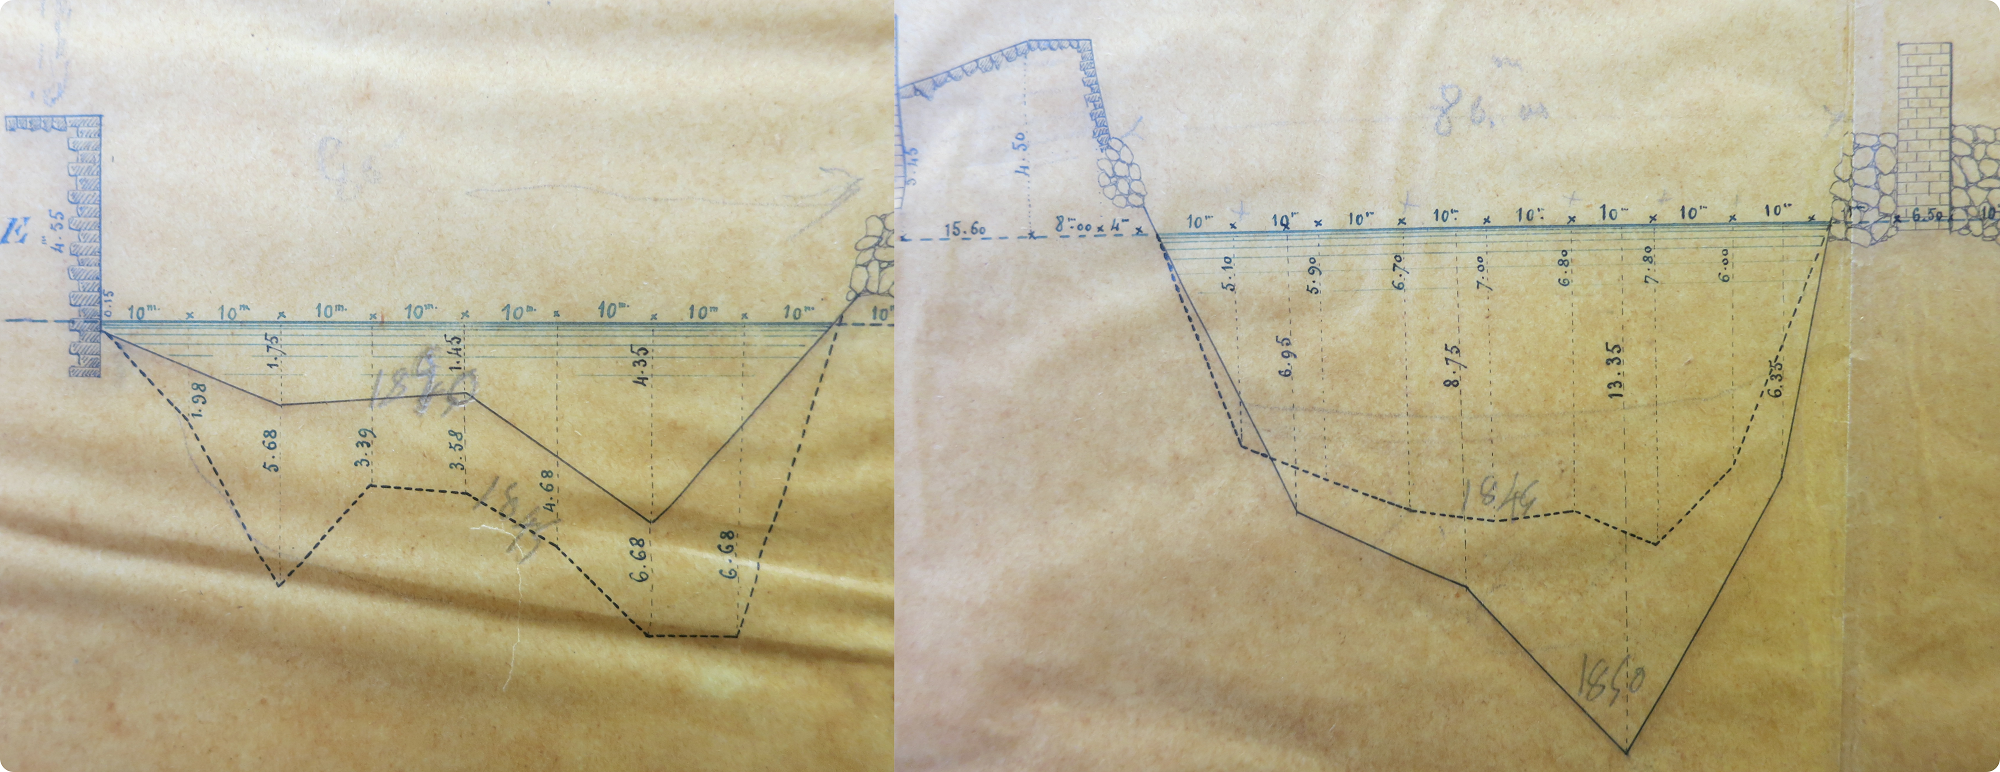
\includegraphics[width = 0.9\linewidth]{Figures/Goux4550.png}
            \caption{Profil en travers du bras de Beaucaire à gauche, et Tarascon à droite, en 1845 (pointillés) et 1850 (trait continu), \citet{goux_modification_1851}. On constate l'approfondissement du bras de Tarascon et le comblement du bras de Beaucaire.}
            \label{fig:ProfGoux}
        \end{figure}
            
        \begin{figure}[h]
            \centering
            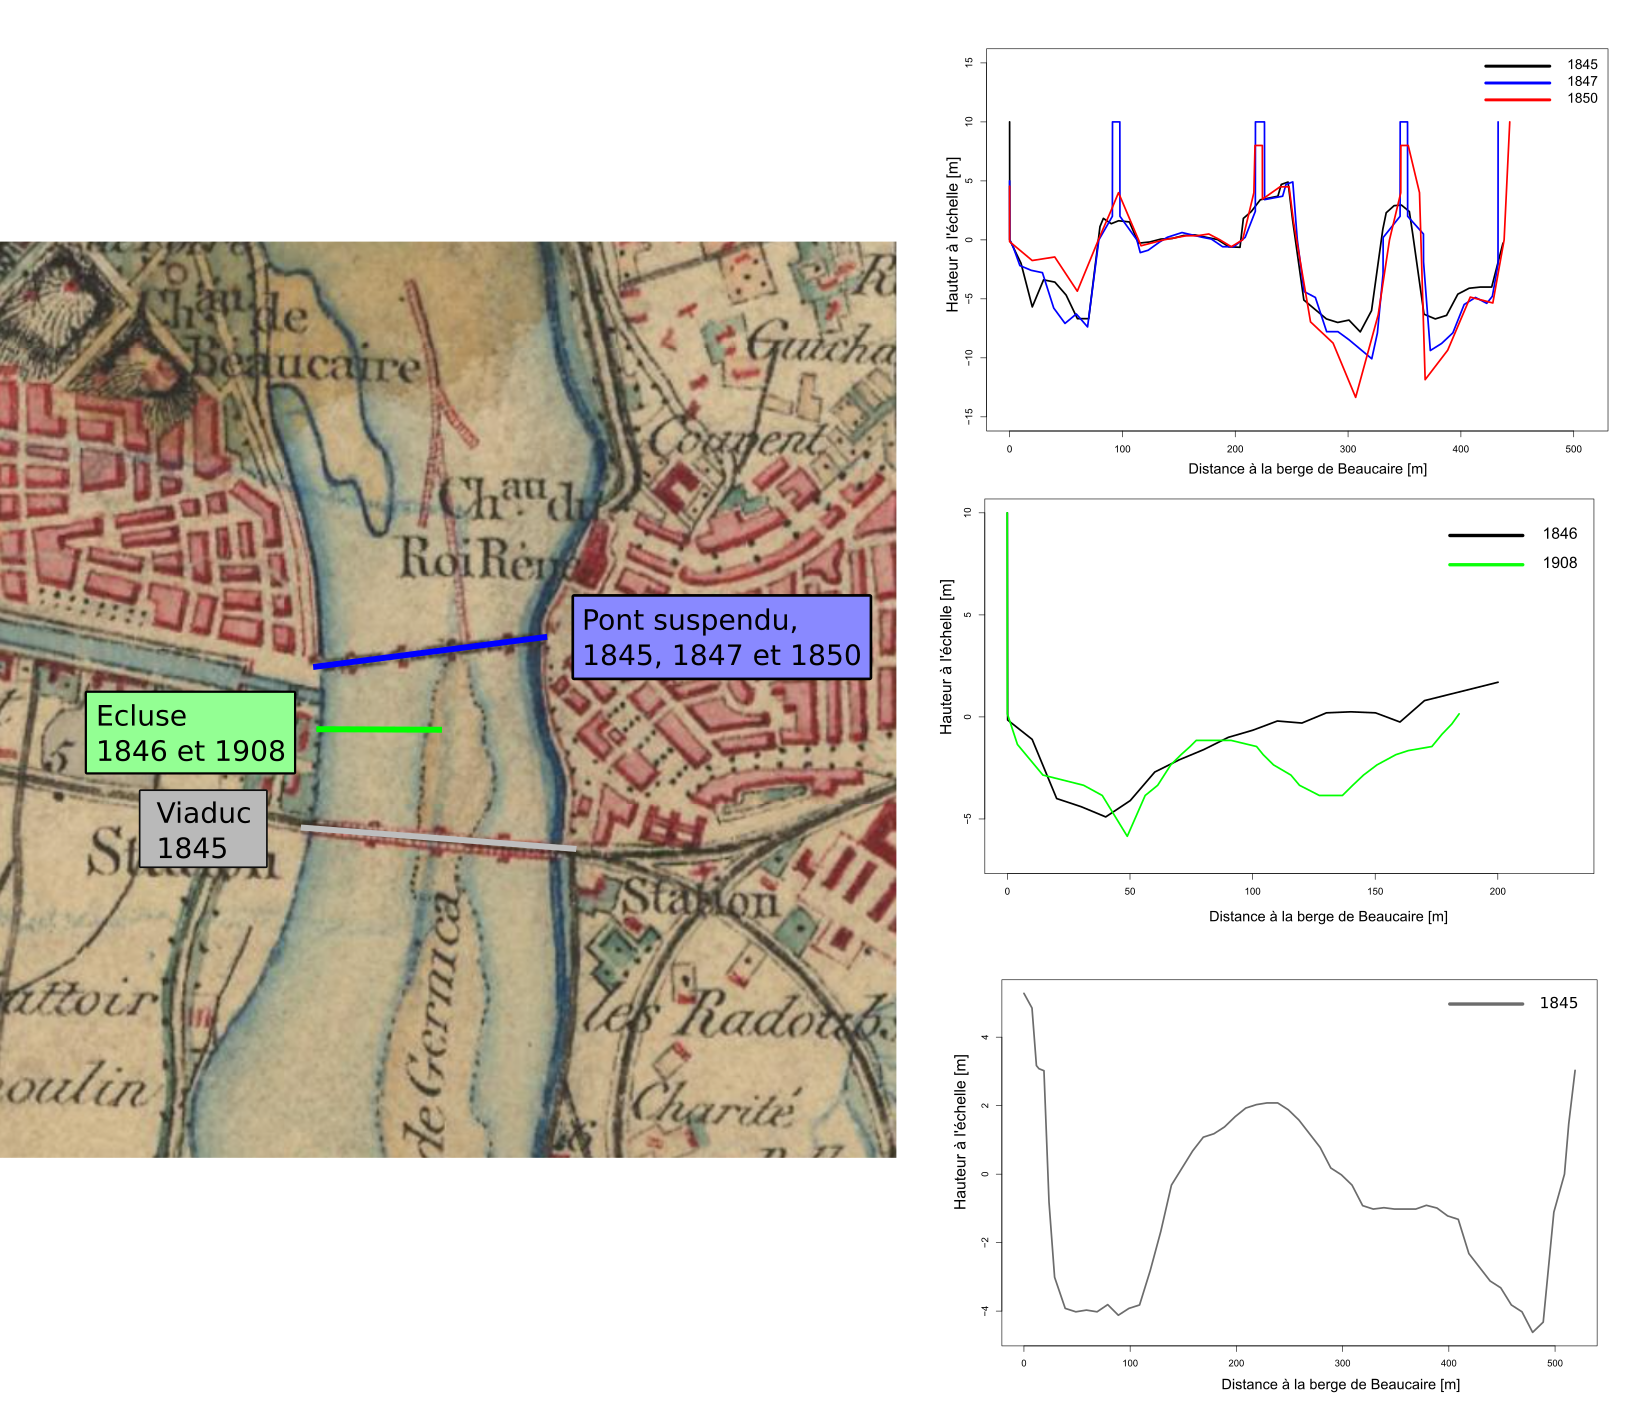
\includegraphics[width = 0.7\linewidth]{Figures/MapProfils.png}
            \caption{Profils en travers XIXème siècle}
            \label{fig:Profis19eme}
        \end{figure}
            
\FloatBarrier
        \paragraph{} Suite à la fixation des deux bras par les digues divisoires vers la fin du XIX\textsuperscript{ème} siècle, on peut supposer qu'il n'y a eu pratiquement aucun changement jusqu'au début des aménagements CNR de Vallabrègues (débutés en 1967 et mis en service en 1970), en témoignent les photos aériennes du portail "Remonter le temps" de l'IGN, de 1936 à 1947 (Figure \ref{fig:AerialBcr}). Ainsi, l'isolement quasi-total du bras de Tarascon au profit du bras de Beaucaire est finalisé en 1884 et a connu de nombreuses phases d'aménagement débutant vers la fin du 18ème siècle. Il est probable qu'à l'époque ancienne, tout comme aujourd'hui, les deux bras communiquaient à haut débit, certainement aux alentours de 6m à l'échelle à l'époque de la finalisation des digues, et à des hauteurs moindres auparavant. Certaines sources signalent par exemple qu'il était ponctuellement possible de traverser en bateau d'un bras à l'autre au niveau de la ville entre 1858 et 1872. Le bras de Beaucaire a sans doute été prépondérant sur le bras de Tarascon sur la majeure partie de l'histoire de la station, excepté la période 1840-1850, en témoignent les profils en travers de \citet{goux_modification_1851} (Figure \ref{fig:ProfGoux}).
    
        \begin{figure}[h]
            \centering
        	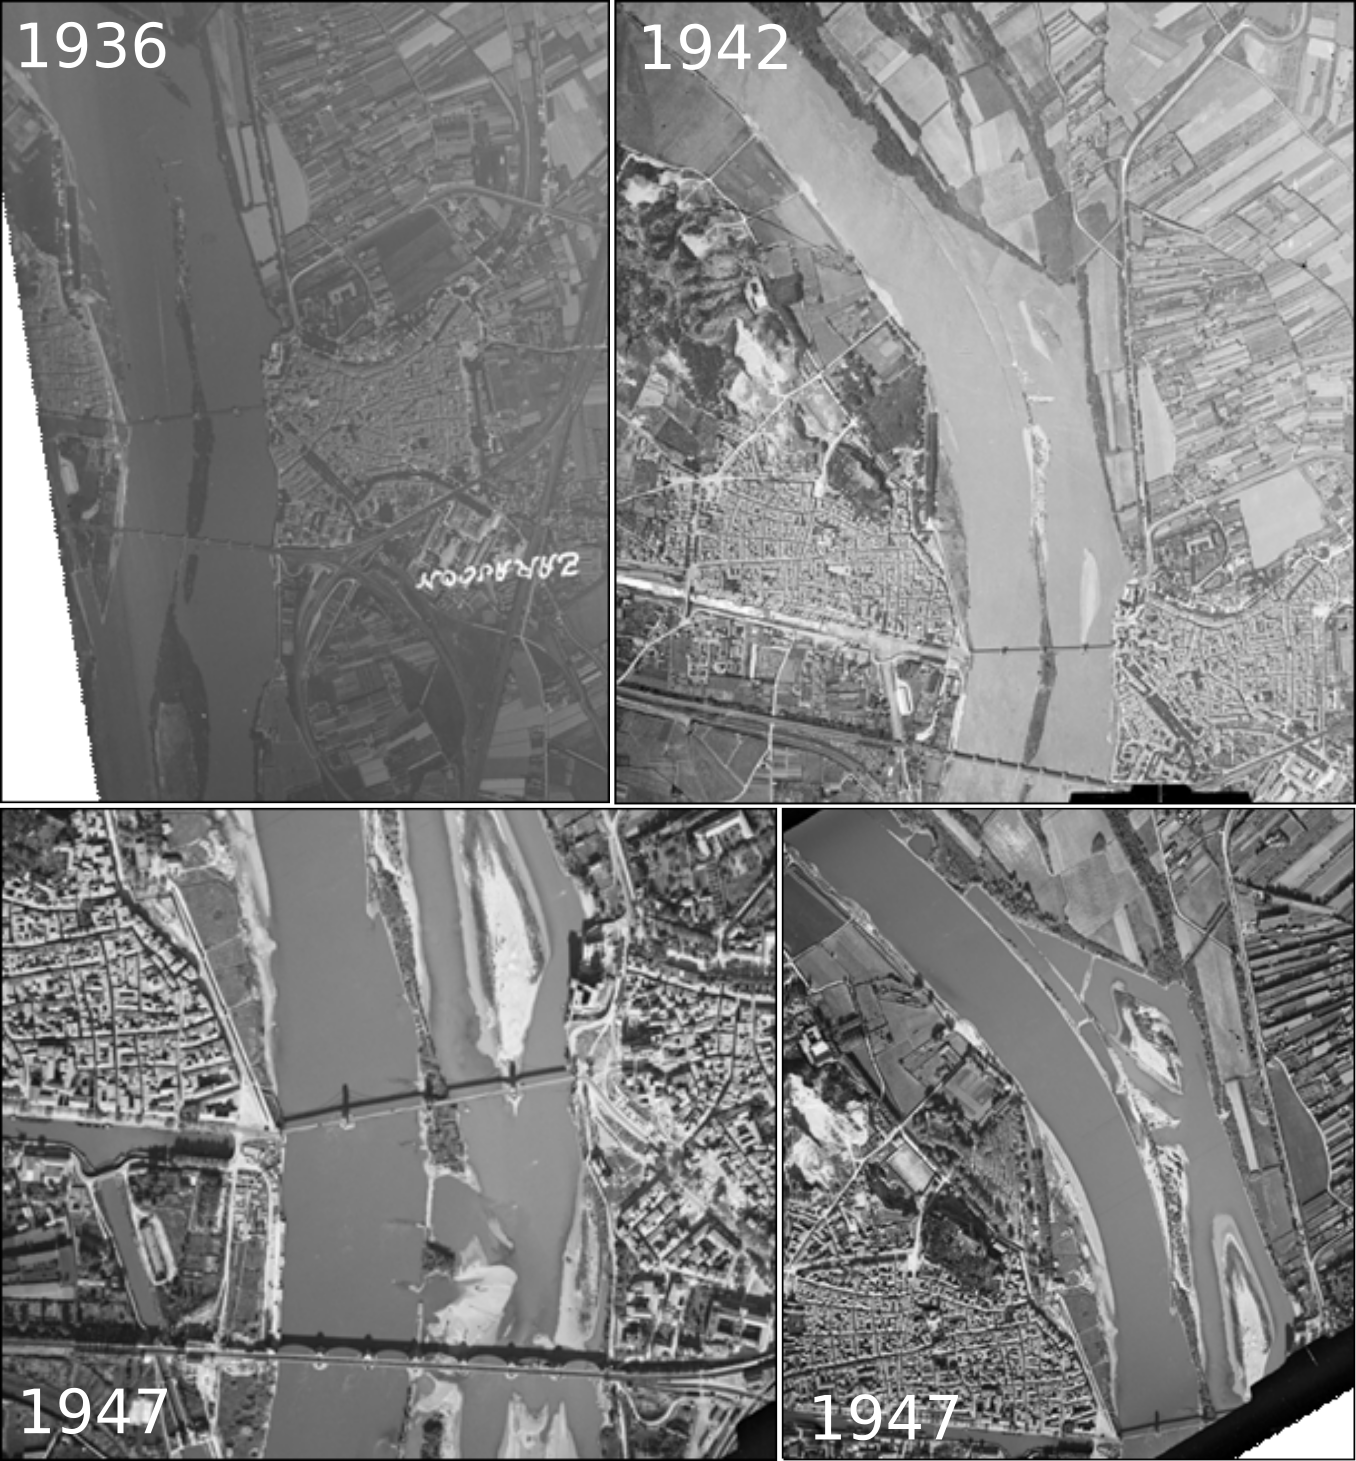
\includegraphics[width = 0.7\linewidth]{Figures/AerialBcr.png}
            \caption{Images aériennes du Rhône à Beaucaire entre 1936 et 1947 (source : www.géoportail.gouv.fr). On remarque la présence des digues sur les 4 images, particulièrement en 1947 pour des débits très faibles.}
            \label{fig:AerialBcr}
        \end{figure}
    
		\paragraph{} Au cours des décades 1860 et 1870, les travaux d'aménagement en lit mineur imaginés par l'ingénieur Girardon sont lancés. Ils permettront de favoriser la navigation fluviale en fixant les berges par l'installation d'épis noyés transversaux sur une grande partie du linéaire du Rhône français. Des épis ont été installés à l'amont et à l'aval de Beaucaire et ont probablement influencé la relation hauteur/débit au droit de la station.
    
		\paragraph{} Les désordres du Rhône à l'aval de Beaucaire étant réguliers avant son endiguement, on imagine que la création des digues a coïncidé avec l'installation des populations dans le secteur, comme attesté par \citet{surell_memoire_1847} : "\textit{Si l'on considère que l'existence de la plaine est presque inévitablement liée à celle des chaussées, on doit croire que celles-ci sont contemporaines de la civilisation même du pays, et qu'elles ont dû occuper, depuis longtemps, les soins de la population}" (les digues étaient fréquemment appelées chaussée dans l'époque ancienne, car elles faisaient également office de voies de circulation). \citet{mejean_etude_2017}, cite l'ingénieur Girard, qui, en 1857, affirme que : "\textit{la construction des premières chaussées entre Beaucaire et Sylvéréal (Camargue) date de l'époque romaine. L'initiative personnelle des propriétaires a ensuite contribué à dresser un système de protection où chacun établissait une levée de terre pour se protéger des invasions du Rhône. La plupart de ces chaussées étaient établies sur les bourrelets alluviaux, car ils présentaient l'avantage d'être déjà surélevés par rapport aux terres voisines. Les chaussées ne présentaient pas une ligne continue de défense, les protections s'établissant autour de quelques grandes propriétés.}" Par la suite, plusieurs grandes phases d'aménagement des digues de protections se sont succédées. Avant le XVI\textsuperscript{ème} siècle, les aménagements étaient discontinus mais deviennent plus organisés avec l'essor de l'agriculture dans les plaines alluviales. Au début du XIX\textsuperscript{ème} siècle, un endiguement continu de Beaucaire à la mer est installé grâce à l'harmonisation des nombreuses associations ou "syndicats des digues", jusqu'alors "\textit{aussi multiples que rivales}" \citep{pichard_sept_2014}. Il protège les populations pour les crues courantes, prétendument jusqu'à la décennale. Au niveau de Beaucaire, la digue de la Montagnette existant depuis le XV\textsuperscript{ème} siècle connut de nombreuses avaries en 1840, 1841, 1843. Des travaux de rehaussement furent effectués en 1843 ainsi qu'en 1883. La digue du chemin de fer (de Tarascon à Arles en rive gauche) vint remplacer en 1846 les digues historiques du Trébon, souvent rompues dans l'histoire. La digue du Trébon était élevée à 6.5 ou 7m au-dessus de l'étiage. La digue du chemin de fer est élevée à 2m10 au-dessus des plus hautes eaux connues à l'époque (1843). Lors de la rupture de la digue de la Montagnette en 1856, Tarascon était enfermée entre Montagnette et le remblai du chemin de fer, l'eau était ainsi restée dans les plaines pendant plusieurs semaines. Ces digues principales furent complétées par des aménagement au sein des villes de Tarascon et Beaucaire entre 1860 et 1866. La "banquette de Beaucaire", constituée d'un mur maçonné construit en 1840 du rocher du château à la chaussée de chemin de fer, fut rehaussée après 1856, puis en 1862 et 1863, environ 2m au-dessus du niveau atteint en 1856. Il en va de même pour les quais de Tarascon et de la digue de la Montagnette, rehaussés en 1860 à 1m50 au-dessus du niveau de 1856.
		
		\paragraph{} Ces nombreuses protections érigées au cours du XIX\textsuperscript{ème} siècle on permis de contenir les crues courantes, puis des crues plus importantes grâce aux aménagements postérieurs aux inondations de 1840 et 1856 qui furent à l'origine d'une prise de conscience illustrée par la création du Service Spécial du Rhône des Ponts et Chaussées. Depuis cette époque, les systèmes de protection n'ont que peu évolué et la crue de 2003 a ravivé les inquiétudes quant au risque de brèches, comme en témoigne cet extrait du rapport du \citet{symadrem_programme_2012} (Syndicat Mixte Interrégional d'Aménagement des Digues du Delta du Rhône et de la Mer) : "\textit{Le système actuel de protection contre les crues du Rhône a été réalisé après les grandes crues de 1840 et 1856. Il est ancien et présente une exposition très forte au risque de brèches. Dans l'état actuel, on estimque que le risque de formation de brèches, confirmé par les crues de 1993, 1994, 2002 et 2003, est quasi-certain à certain}". Depuis la crue de 2003, un programme de sécurisation a été réalisé, prévoyant notamment la réalisation de digues résistantes à la surverse et à la formation de brèches (REF SYMADREM).    
		
		\subsubsection{Évolution géomorphologique}
		
		SECTION TIREE DE BARD ET LANG, A REVOIR
		
		\paragraph{} Il est évident que les conditions d’écoulement du Rhône ont varié depuis l’implantation de la station hydrométrique de Beaucaire. D’une part l’évolution naturelle du transport sédimentaire depuis la fin du petit Age glaciaire, et d’autres part les nombreux aménagements réalisés sur le fleuve au XIXème et XXème siècles : à la fois dans le lit mineur pour la navigation et la stabilisation des berges mais aussi dans la plaine d’inondation par l’érection ou le renforcement de digues contre les inondations, sans compter les modifications du transit sédimentaire sur le Rhône et ses affluents au gré des aménagements hydro-électriques.
La thèse menée par Guillaume Raccasi (2008) sur les mutations géomorphologiques du Rhône aval apporte de nombreux éléments qui sont ici repris pour éclairer l’évolution des conditions hydrauliques à Beaucaire :

\paragraph{} La plaine d’inondation entre les digues insubmersibles, homogénéisées dans les années 1850-90, affiche une stabilité globale sur une période de 150 ans (1876-2003). Entre Beaucaire et Arles les différences d’hydraulicité du lit majeur sur cette période sont minimes. En amont du défilé de Beaucaire, dans la plaine de Vallabrègues-Boulbon les dépôts alluvionnaires de crue sont un peu plus importants (3.7 106 m3) et lissent les irrégularités topographiques.
\paragraph{}Le chenal et ses marges sont au contraire caractérisés par une importante mobilité morphologique de Beaucaire à la mer. Elle correspond d’abord à une métamorphose fluviale, puis à une rétraction généralisée du chenal, en réponse principalement aux aménagements du fleuve :
\begin{itemize}
	\item{}Premiers ouvrages (digues, épis) dans les années 1860-70, atterrissement des bancs, incision du chenal notamment au droit de la lône du Pillet (PK 274), fixation de la diffluence Petit Rhône / Grand Rhône, rétractation du chenal sur le seuil de Terrin (PK 294 Grand Rhône) ;
	\item{}Simplification du chenal en amont du PK 276 avant 1905 et dans la première moitié du XXème en aval de ce point ;
	\item{}Rétractation du chenal, avec fermeture complète des lônes et alluvionnement des marges, qui se prolonge au XXème voire s’accélère depuis 1960.
\end{itemize}

\paragraph{}L’incision du plancher alluvial affecte tout le chenal de Beaucaire à la mer, avec une sectorisation nette : importante en amont du PK 276 puis modeste jusqu’à la diffluence. Sur le Petit Rhône, elle est plus importante en amont de l’écluse de St-Gilles, puis diminue ensuite.

\paragraph{}Le secteur en amont de la diffluence reste à l’heure actuelle une zone de dépôt dans le chenal qui fait l’objet de draguages

\FloatBarrier
	\subsection{Station hydrométrique du Rhône à Beaucaire restitution (1970-aujourd'hui)}
	
	\subsubsection{Données disponibles}

	\paragraph{} La station de Beaucaire restitution (PK 269.6) a pris le relais sur la station de Pont de Beaucaire suite aux travaux de l'aménagement hydroélectrique de Vallabrègues, et de l'installation d'un chenal de dérivation restituant une partie du débit à l'aval de la ville de Beaucaire. La nouvelle station fut alors installée 2 km plus à l'aval, environ 600 m à l'aval de la restitution des débits transitant par la centrale hydroélectrique CNR (figure \ref{fig:CartoRes}). Durant les travaux, de 1967 à 1970, les débits de la Durance ayant été dérivés vers l'étang de Berre, les relevés des deux stations sont considérés comme manquants. La station de Beaucaire Restitution demeure au même emplacement depuis sa mise en service en 1970. Elle est équipée dès sa création de capteurs automatiques réalisant des relevés au pas de temps infra-horaire. L'ensemble de ces relevés, ainsi que les jaugeages réalisés à la station, sont disponibles au sein des bases de données de la CNR.
		
	\begin{figure}[h]
	\centering
		\includegraphics[width=.7\linewidth]{Figures/RestitCartoPh.png}
        \caption{Gauche : Localisation de la station de Beaucaire restitution (carte IGN Scan25, source : www.geoportail.fr). Droite : échelle limnimétrique de Beaucaire restitution en Février 2020.}	
		\label{fig:CartoRes}
	\end{figure}
	
	
		\subsubsection{Évolution morphologique}

	\paragraph{} La section du Rhône au niveau de la station de Beaucaire restitution a connu de nombreux dragages des matériaux du fond du lit suite à la construction de l'aménagement de Vallabrègues, durant les 5 années après la mise en service du système en 1970, ainsi qu'en 1997 et 1998 suite à la construction du nouveau pont routier de Beaucaire. En dehors de ces interventions, le profil au droit de la station est stable (figure \ref{fig:ProfilsRestit}). 
	
	\begin{figure}[h]
	\centering
		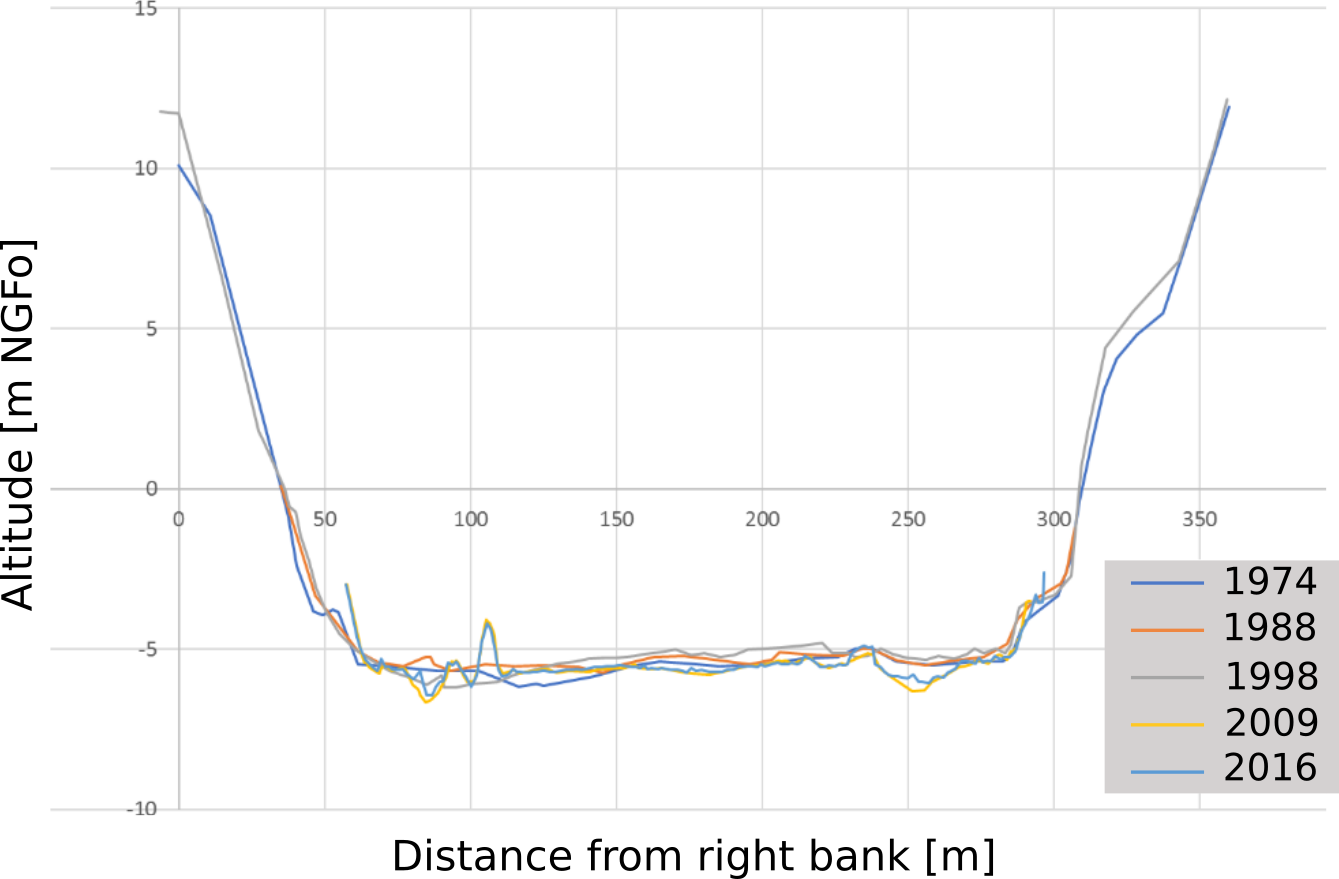
\includegraphics[width=.6\linewidth]{Figures/ProfilsBardRestit.png}
        \caption{Profils en travers du Rhône à la station de Beaucaire restitution réalisés par la CNR entre 1974 et 2016. Adapté de \cite{bard_actualisation_2018}.}	
		\label{fig:ProfilsRestit}
	\end{figure}
	
       
\FloatBarrier


\section{Données historiques : la base de données HISTRHÔNE (1300-2000)}

	\subsection{Présentation de la base de données}

	\paragraph{} La base de données HISTRHÔNE (histrhone.cerege.fr) \citep{pichard_sept_2014} regroupe près de 1500 événements hydro-climatiques, depuis le XIII\textsuperscript{ème} siècle jusqu'à l'an 2000. Cet important travail d'archives qui s'est étalé sur plusieurs décennies, représente un apport majeur pour la connaissance de l'histoire climatique de la basse vallée du Rhône. La zone couverte par la base de données s'étale de la ville de Pont Saint-Esprit jusqu'à la mer Méditerranée, en incluant les villes d'Avignon, Beaucaire et Arles, ainsi que l'ensemble de la Camargue (figure \ref{fig:MapHistrhone}). 
	
	\begin{figure}[h]
	\centering
		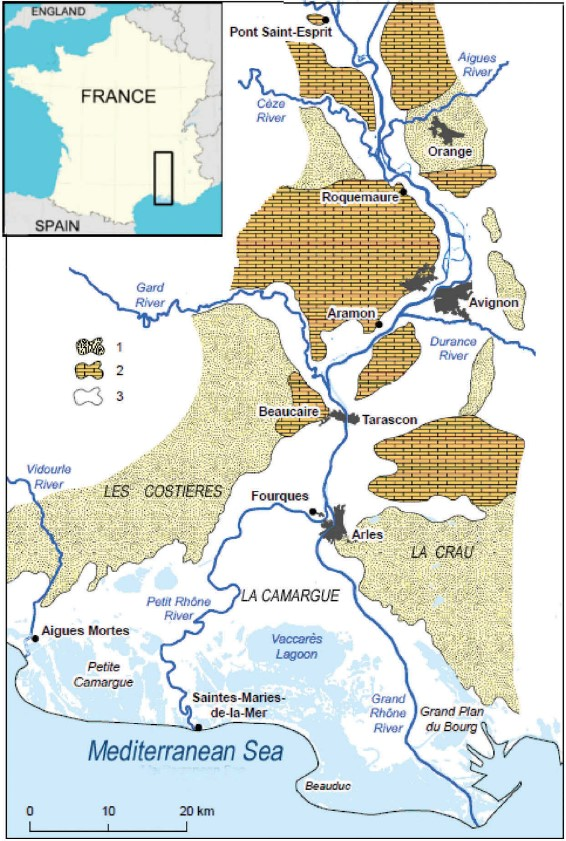
\includegraphics[width=.5\linewidth]{Figures/HistrhoneMap.jpg}
        \caption{Localisation de la zone géographique couverte par la base HISTRHÔNE \citep{pichard_sept_2014} }
		\label{fig:MapHistrhone}
	\end{figure}
	
	\paragraph{} Les éléments historiques (témoignages, cartes...) qui correspondent à un même événement hydroclimatique sont regroupés et ces événements sont classés par type dans la base de données : crue, étiage, présence de glace ou gel du Rhône, inondation pluviale, submersion marine... Au delà de la base de données, l'ouvrage "\textit{Sept siècles d'histoire hydroclimatique du Rhône d'Orange à la mer}" \citep{pichard_sept_2014} "\textit{offre une vue synoptique, à la fois des sources, de leur critique et des perspectives ouvertes par les premiers résultats que les auteurs ont pu en tirer comme contribution à une histoire hydroclimatique}". Il faut ajouter qu'une chronologie générale des événements est disponible, ainsi qu'une étude détaillée des échelles limnimétriques du bas Rhône qui "\textit{reprend l'ensemble des problèmes de mesures de hauteurs des crues dans l'histoire et tente de résoudre ces complications pratiques de métrologie}" \citep{pichard_hauteurs_2013} .
	
	\paragraph{} Dans la base de données HISTRHÔNE, les événements de crues sont classés en 6 catégories présentées dans le tableau \ref{tab:CatCrueHistrhone}. Ces catégories correspondent à différents niveaux de gravité, allant d'un Rhône "pleins bords" jusqu'à l'inondation extraordinaire. D'après \citet{pichard_sept_2014}, ces catégories permettent le classement des crues même en l'absence d'informations sur les hauteurs ou les débits : "\textit{Un seuil de hauteur unique présente l'intérêt de la simplicité et de l'universalité. On peut ainsi choisir la limite évidente du débordement hors du lit mineur, surtout si cette limite est bien connue et sans ambiguïté, mais il faut alors renoncer à pondérer des types de crues que les sources anciennes ne permettent pas de discriminer. [...] il faut se résoudre à choisir le type de crue en fonction de critères indirects, mais tout aussi pertinents que les hauteurs et les débits. On s'appuie sur la comparaison avec la période des hauteurs mesurées en continuité, mais aussi sur les conséquences et les dommages, sur l'extension de la crue dans la plaine proximale ou distale, sur sa généralisation dans une partie ou la totalité du territoire étudié}". Si la détermination d'un seuil de hauteur ou de débit n'est donc pas essentiel pour l'analyse de l'historique hydroclimatique, il l'est en revanche pour l'utilisation de ces données dans le cadre de l'analyse fréquentielle des crues.  Il faudra donc veiller à la correspondance entre ces catégories basées sur des informations très diverses, et un éventuel seuil de perception.
	
\begin{table}[h]
	\centering
	\caption{Classification des événements de crues de la base HISTRHÔNE. Les estimations de débit proviennent de \citet{pichard_hydro-climatology_2017}.}
	\label{tab:CatCrueHistrhone}
%	\resizebox{\columnwidth}{!}{
		\begin{tabular}{|m{1cm}|m{5cm}|m{8cm}|m{2.5cm}|}
		\hline
		Code &
		  Libellé &
		  Description &
		  Débit estimé \\ \hline
		Ci &
		  Crue de gravité indéterminée &
		  Crue sans aucune précision : pas d'indice de débordement ni de gravité (incertitude totale) &
		  9000 m\textsuperscript{3}/s \\ \hline
		Cd &
		  Crue avec indice de débordement &
		  Débordement avéré mais sans précision relative à son étendue ou sa gravité (incertitude partielle) &
		  7200 m\textsuperscript{3}/s \\ \hline
		C1 &
		  Hautes eaux &
		  
\textbf{Rhône "pleins bords", "gros Rhône" sans débordement}. Le Rhône reste dans son lit mineur mais implique une surveillance constante aux digues &
		  5200 m\textsuperscript{3}/s \\ \hline
		C2 &
		  Crue avec débordement sans gravité et/ou localisé &
		 
\textbf{Débordement limité}, sans gravité majeur ou bien localisé (ségonnaux, prés/chemins inondés, eaux sur les quais, dégâts mineurs sur digues) &
		  X \\ \hline
		C3 &
		  Crues et inondation de gravité intermédiaire &
		  
\textbf{Inondation notable} avec dégâts avérés au caractère destructeur et/ou extension de crue &
		  X \\ \hline
		C4 &
		  Crue et inondation extrême &
\textbf{Inondation extraordinaire} avec dégâts exceptionnels (pertes humaines et animales, intérieurs des villes inondés, dégradations de digues en grand nombre) et extension de crue &
		  X \\ \hline
		\end{tabular}
%	}
\end{table}
	
\FloatBarrier

	\subsection{Ordre de grandeur des crues de la base HISTRHÔNE}
	
	\paragraph{} L'exploitation des crues historiques pour l'analyse fréquentielle nécessite d'estimer un ordre de grandeur du débit de ces événements. Plus précisément, il est possible d'exploiter statistiquement les données historiques à condition d'en déterminer un seuil de perception. Il s'agit ici de garantir que toutes les crues dont le débit fut supérieur à un seuil de perception ont laissé une trace dans les archives. Dans le cas des événements de la base HISTRHÔNE, il est possible de faire correspondre un seuil de perception à chacune des catégories. L'analyse fréquentielle des crues qui découle de ces seuils de perception sera réalisée au chapitre 4 (REF), mais il faut tout d'abord en faire une première estimation. \citet{pichard_hydro-climatology_2017} en donne un premier ordre de grandeur (table \ref{tab:CatCrueHistrhone}) en calculant la moyenne du débit à Beaucaire des crues de chaque catégorie pour les événements du XX\textsuperscript{ème} siècle, en utilisant les données de la banque hydro (\url{www.hydro.eaufrance.fr}). Néanmoins, l'utilisation d'une moyenne ne reflète pas exactement le concept de seuil de perception présenté plus tôt, mais cela permet d'en connaitre l'ordre de grandeur. Le débit de la plus petite crue de chacune des catégories serait plus adapté. 
	
	\begin{figure}[h]
	\centering
		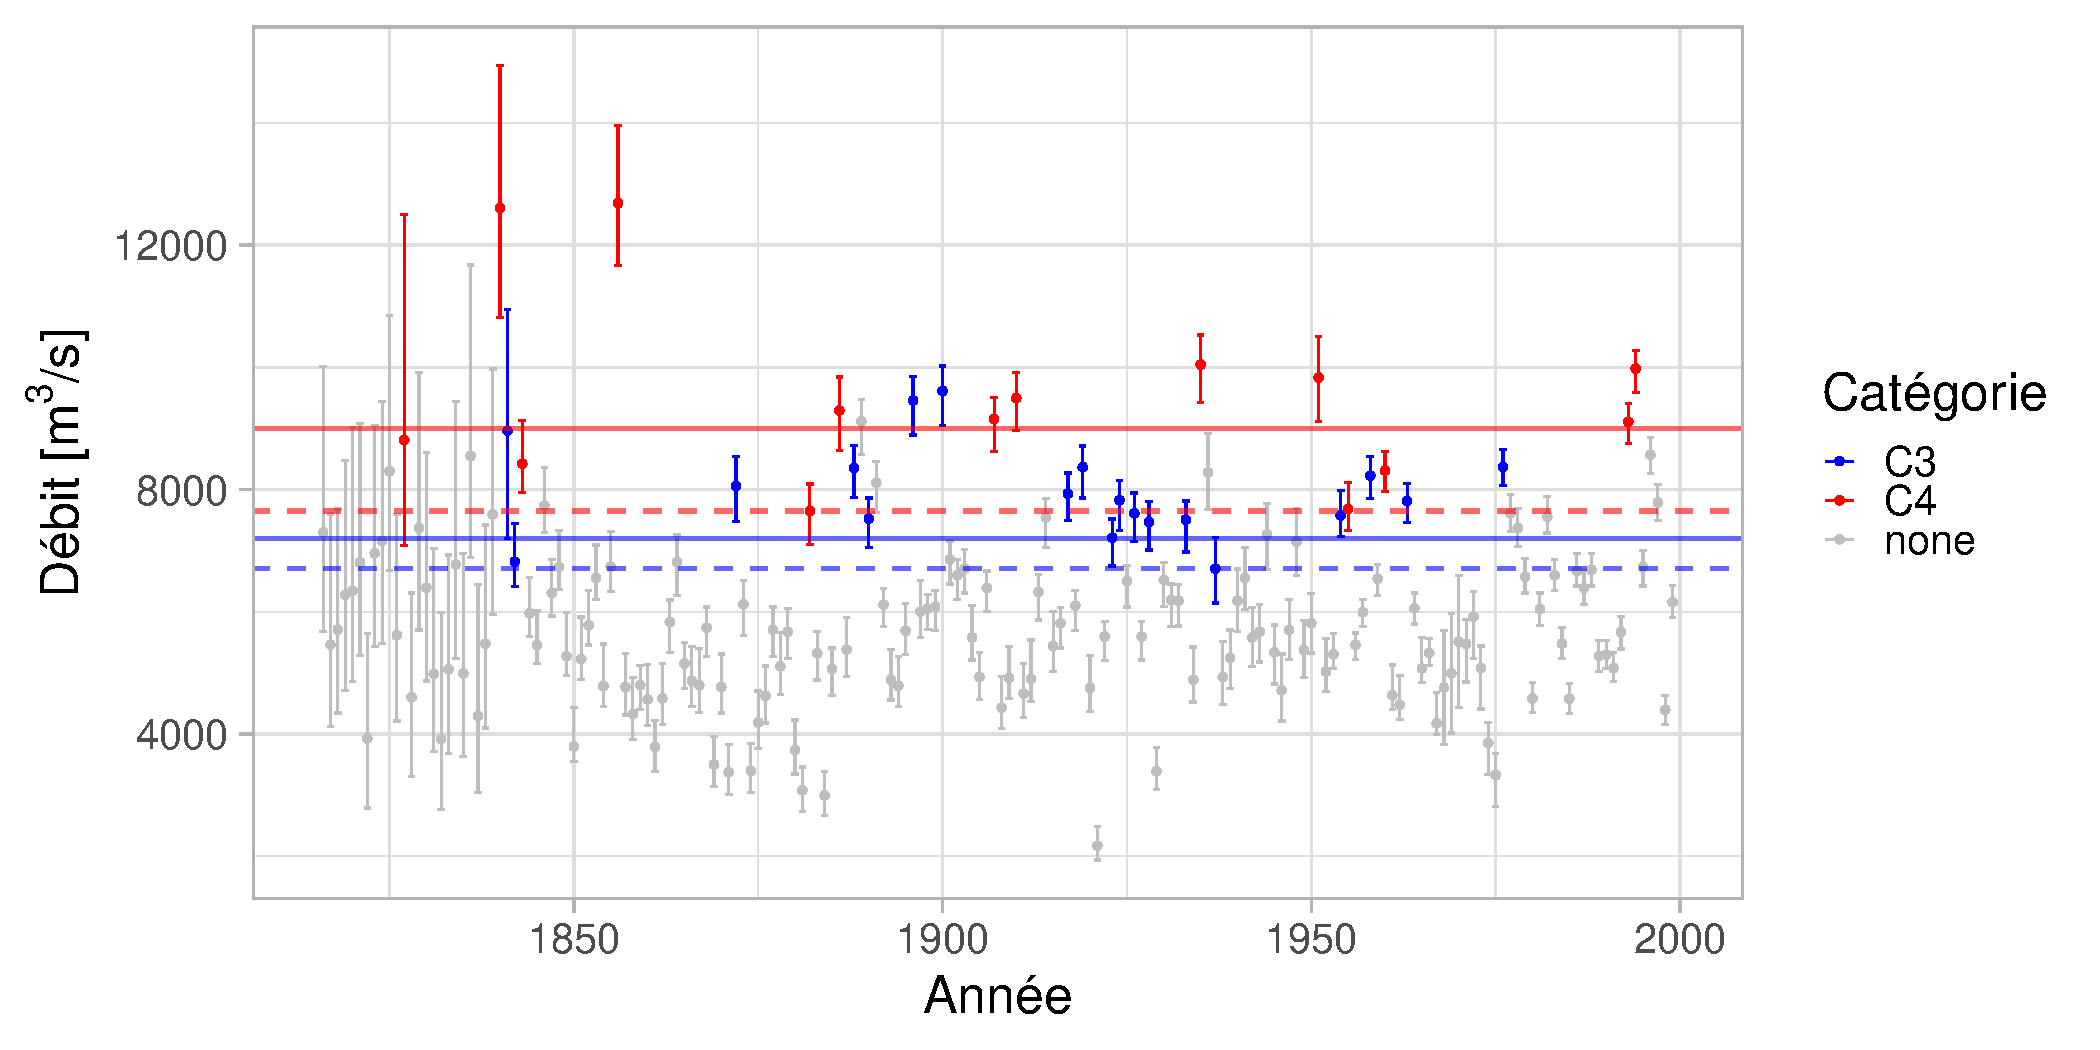
\includegraphics[width=.9\linewidth]{Figures/C3-C4_SystematicPeriod-FR.pdf}
        \caption{Débit maximum annuels à Beaucaire de 1816 à 2020 (estimations chapitre 3 REF). Les barres d'erreur représentent l'incertitude à 95\%, les droites horizontales représentent l'estimation de \citet{pichard_hydro-climatology_2017} (trait plein) et le débit maxpost de la plus petite crue de chacune des catégories (trait pointillé).}
		\label{fig:C3-C4_Syst}
	\end{figure}
		
	
	\paragraph{} Les débits maximum annuels avec incertitude de 1816 à 2020 calculés au chapitre 3 (REF) sont croisés avec les catégories C3 et C4 de la base HISTRHÔNE. Seules ces deux catégories sont retenues car elles contiennent des crues responsables de dégâts notables et sont susceptible d'être informatives pour l'analyse fréquentielle menée au chapitre 4 (REF). On remarque sur la figure \ref{fig:C3-C4_Syst} que les limites entre catégories sont "perméables", du moins pour cette période "témoin" de 1816 à 2000 : des crues appartenant à la catégorie C3 sont plus fortes que certaines crues de la catégorie C4. \citet{pichard_sept_2014} explique que : "\textit{Ce sont les catégories C3 et C4 qui offrent les plus grandes difficultés de discrimination. Pour la catégorie C3, la distinction avec les crues localisées est parfois délicate [...] Il y a une gradation certaine au sein de cette catégorie [...] Ce sont ainsi les crues dites extrêmes qui permettent de délimiter les passage dans la catégorie supérieure, beaucoup plus nette. Les crues extrêmes (C4) entrainent des destructions importantes, s'introduissent au cœur des villes et dans les maisons, couvrent des territoires les plus étendus et transforment la Camargue et le Plan du Bourg d'Arles en mers à perte de vue.}" De plus, certaines crues ne sont pas classées bien que supérieures à certaines crues C4.	
	
	\paragraph{} La moyenne des crues de chaque catégorie sur la période 1816-2000 est plus forte que celle présentée par \citet{pichard_hydro-climatology_2017} car cette dernière est calculée uniquement sur les données XX\textsuperscript{ème} siècle (table \ref{tab:Qcateg}). Ces valeurs moyennes permettent d'avoir un ordre de grandeur du débit de ces catégories mais ne répond pas à la définition du seuil de perception. Le débit de la plus petite crue de chaque catégorie représente une estimation plus adéquate, même si les limites entre catégories ne semblent pas univoques en terme de débit. Ces constatations encouragent la considération d'une incertitude autour du seuil de perception. De plus, le fait que certains débits maximum annuels supérieurs à la plus petite des crues C4 (1816-2000) ne correspondent à aucune des deux catégories encourage à la méfiance quand à l'exhaustivité des données sur l'ensemble de la période. Il semble optimiste que l'incertitude du seuil de perception soit choisie égale à l'incertitude de la plus petite crue de la période 1816-2000, celle-ci étant relativement faible (figure \ref{fig:C3-C4_Syst}) et ne représentant pas de manière satisfaisante la méconnaissance du seuil. Le choix d'une distribution plus large incluant l'ensemble des valeurs du tableau \ref{tab:Qcateg} semble être un choix plus pragmatique.	

	\begin{table}[h]
	\centering
	\caption{Débits caractéristiques des catégories de la base HISTRHÔNE. Les estimations de \citet{pichard_hydro-climatology_2017} représentent la moyenne des débits maximum annuels du XX\textsuperscript{ème} siècle. Les autres colonnes correspondent à la moyenne des débits maximum annuels de chaque catégorie et le débit de la crue la plus petite de chacune des catégories basés sur la chronique continue estimée de 1816 à 2000 au chapitre 3 (REF).} 
	\label{tab:Qcateg}
		\begin{tabular}{|c|c|c|c|}
		\hline
		Catégorie HISTRHÔNE & \citet{pichard_hydro-climatology_2017} & Moyenne 1816-2000 & Minimum 1816-2020\\ \hline
		C3  & 7200 m\textsuperscript{3}/s  & 7970 m\textsuperscript{3}/s    & 6706 m\textsuperscript{3}/s   \\ \hline
		C4  & 9000 m\textsuperscript{3}/s  & 9506 m\textsuperscript{3}/s    & 7649 m\textsuperscript{3}/s   \\ \hline
		\end{tabular}
	\end{table}
	
	\subsection{Évolution temporelle de la vulnérabilité aux inondations}
	
	\paragraph{} Le classement des crues dans la base HISTRHÔNE est basé sur des critères indirects, différents du débit et de la hauteur d'eau, tels que : "\textit{les conséquences et les dommages, sur l'extension de la crue dans la plaine proximale ou distale, sur sa généralisation dans une partie ou la totalité du territoire étudié}" \citep{pichard_sept_2014}. Les mêmes critères sont utilisés pour catégoriser les crues du XIV\textsuperscript{ème} siècle et celles du XX\textsuperscript{ème} siècle. Pourtant, la vulnérabilité des populations ripariennes évolue au cours du temps, et ce partout dans le monde (REF Kron 2002). De nombreux exemple de cette évolution existent, y compris en France, comme démontré par \citet{boudou_assessing_2016} pour les bassins versants du Doubs et du Tarn. La basse vallée du Rhône ne fait pas exception à la règle (REF OSR 2022). De plus, la perception des dommages par les populations est elle aussi variable et est la conséquence de nombreux facteurs, pouvant être d'origine physique (niveau de protection aux inondations, rupture de digues, densité de populations...), médiatiques (contexte sociétal, politique, religieux...). Ainsi, on observe au sein des données de crues de la base HISTRHÔNE des fluctuations dont l'origine n'est pas seulement climatique. 
	
	\begin{figure}[h]
	\centering
		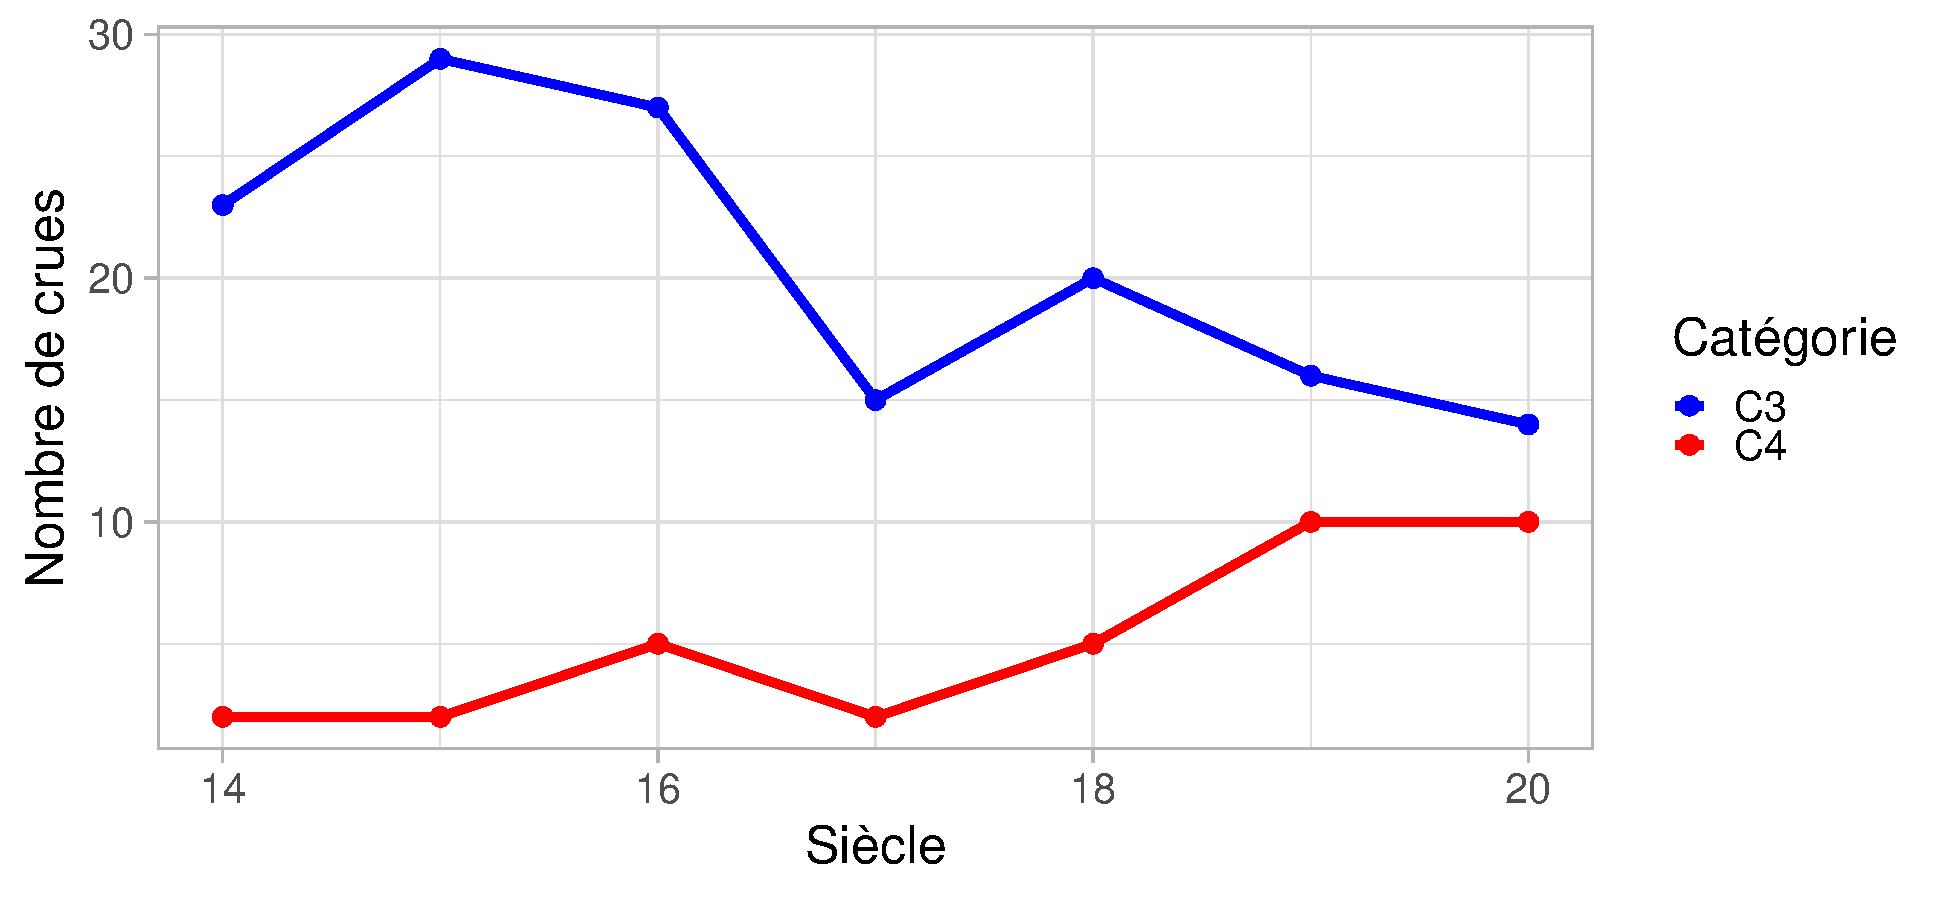
\includegraphics[width=.8\linewidth]{Figures/Nb_C3-C4.pdf}
        \caption{Nombre de crues par siècle dans les catégories C3 et C4 de la base HISTRHÔNE, du XIV\textsuperscript{ème} au XX\textsuperscript{ème} siècle.}
		\label{fig:Nb_C3C4}
	\end{figure}	
	
	\paragraph{} La figure \ref{fig:Nb_C3C4} témoigne de l'évolution de la perception des crues des catégories C3 et C4. On constate une diminution du nombre de crues C3 à partir du XVII\textsuperscript{ème} siècle, au profit des crues de la catégorie C4. Plusieurs facteurs peuvent expliquer cette évolution. \citet{pichard_sept_2014} l'attribuent notamment aux actions anthropiques : "\textit{La reconstruction et l'extension des digues, le défrichement des rives, l'essor urbain, tout concourt à concentrer les écoulements lors des plus grands épisodes tout en atténuant ou même en faisant disparaître les débordements ordinaires ou moyens (C2 et C3)}".
	

\section{Estimation du débit des événements historiques}

	\paragraph{} Dans l'optique de l'utilisation des données de crues historiques de la base HISTRHÔNE pour l'analyse fréquentielle, la connaissance du débit de chacun des événements peut s'avérer utile. Cependant, l'estimation de ces débits dans un contexte historique est bien plus complexe que dans le cas de stations hydrométriques. Plusieurs zones d'ombre viennent complexifier ces estimations. Tout d'abord, la mesure limnimétrique n'est pas continue et repose sur des témoignages sporadiques donnant des informations très dispersées spatialement. Il peut être complexe de reconstituer la hauteur d'eau correspondant à la pointe de la crue et il est encore plus complexe de reconstituer la dynamique temporelle de la crue. Ensuite, la transformation hauteur/débit est complexifiée en l'absence de jaugeages et complexifie l'estimation d'une courbe de tarage. Le schéma hydrométrique classique ne peut donc être suivi. Une des solutions est l'utilisation d'un modèle hydraulique. Cependant, son utilisation est conditionnée à l'existence ou à la reconstitution de données topographiques et bathymétriques contemporaines à la crue étudiée. La modélisation hydraulique unidimensionnelle (1D) est très simplifiée car elle fait l'hypothèse que les quantités (hauteur d'eau, vitesses et direction de l'écoulement) sont uniformes au sein d'une section en travers. Ce type de modèle n'est pas aussi précis qu'un modèle 2D, mais il demande en revanche une description bien moins fine de la géométrie de la rivière, ce qui est avantageux dans le cas de reconstitution historiques pour lesquelles ces données sont rares. La modélisation hydraulique des événements historiques a été explorée mais n'a pas abouti par manque de temps et de données bathymétriques anciennes. Les grandes lignes du travail effectué sont décrites dans la section suivantes et peuvent être utile à qui envisagera de modéliser les crues historiques du bas-Rhône. Des hypothèses simplificatrices du modèle hydraulique sont notamment explorées afin de limiter la quantité d'informations nécessaires dans le cadre de modélisations historiques.
	
	\epigraph{"\textit{Je ne dirais pas que c'est un échec. Ça n'a pas marché.}"}{Emmanuel Macron le 14 Octobre 2020}
	
	 \subsection{Adaptation du modèle MAGE OSR 1D à l'étude des crues historiques à Beaucaire}
	 
	 \paragraph{} L'Observatoire des Sédiments du Rhône (OSR) (\url{www.graie.org/osr}) étudie les flux sédimentaires ainsi que les pollutions associées à ces sédiments sur la partie française du Rhône. A ce titre, un modèle hydraulique à été développé sur l'ensemble du linéaire. Ce modèle se base sur le code de calcul MAGE (REF MAGE ?) qui résout les équations de Barré-de-Saint-Venant 1D ainsi que la formule de perte de charge de Manning-Strickler. Ce modèle représente les 545 km du linéaire français du Rhône, du lac Léman à la Méditerranée. Il inclut également les tronçons les plus à l'aval des principaux affluents, ainsi qu'une représentation simplifiée des aménagements hydroélectriques. Il a été calé et validé jusqu'au débit des crues non débordantes (soit un débit de période de retour d'environ 10 ans pour la partie à l'aval de Lyon). La géométrie du lit est définie par des profils en travers réalisés environ tous les 500 m. Le modèle n'étant pas prévu pour représenter les crues débordantes, les profils en travers s'étendent jusqu'aux limites du lit moyen, aussi appelé lit majeur actif (c'est à dire la partie mouillée pour les crues fréquentes). Les débordements ne sont donc pas pris en compte et la géométrie au delà de la berge est représentée par des murs verticaux artificiels dont les frottements sont négligés. 
	 
	 \paragraph{} Le modèle MAGE OSR 1D est adapté à l'étude de la dynamique hydro-sédimentaire, mais ne peut en l'état être utilisé pour la modélisation des crues : plusieurs adaptations et hypothèses simplificatrices sont nécessaires. Tout d'abord, il est inutile de conserver la totalité des biefs, le modèle s'étendant du lac Léman à la Méditerranée. Afin de limiter la quantité de données topographiques anciennes nécessaire et le temps de calcul, la limite amont du modèle est dans un premier temps définie à l'aval immédiat de la confluence avec la Durance (figure \ref{fig:MAGEavap}, gauche). A l'aval de la Durance, la confluence avec le Gardon (dernier affluent du Rhône) est représentée par un apport latéral et ne nécessite donc pas de reconstituer la bathymétrie de l'affluent. La limite aval originelle du modèle est représentée par la mer Méditerranée pour les deux biefs du delta, Petit et Grand Rhône. Étant donné la complexité de reconstituer les fortes évolutions bathymétriques de l'embouchure du grand Rhône (figure \ref{fig:Embouch}), la limite aval du modèle sur ce bief peut être fixée plus à l'amont. Il existe un nombre important de hauteurs d'eau pour les crues historiques à l'échelle reconstituée des marches du port d'Arles \citep{pichard_les_1995}, la limite aval est donc fixée au niveau de cette échelle, au PK 282.2. 
	
	\begin{figure}[h]
		\centering
	    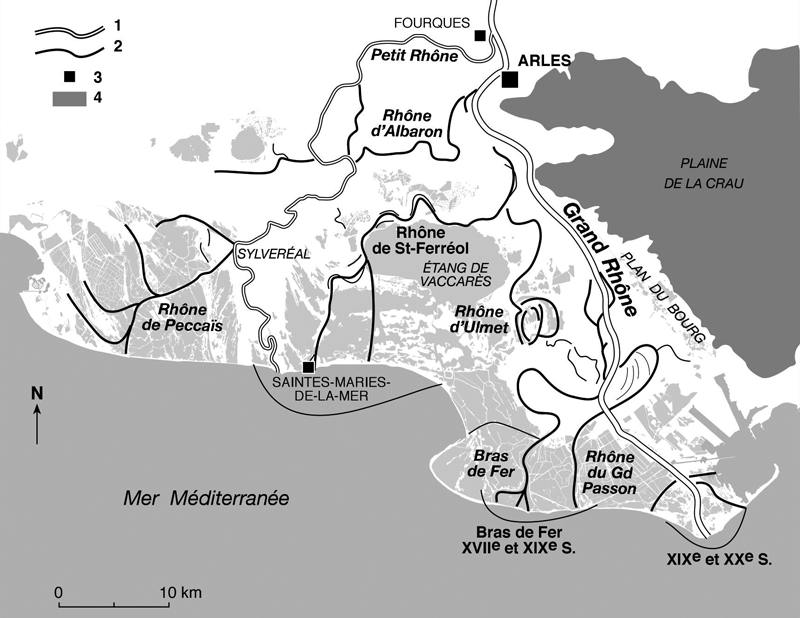
\includegraphics[width=.8\linewidth]{Figures/EvolEmbouch.jpg}
        \caption{Évolutions morphologiques du delta du Rhône du XIV\textsuperscript{ème} à aujourd'hui (REF PICHARD). 1 : bras actifs de nos jours, 2 : tracés des bras hérités, 3 : Principales localités, 4 : plateau de Crau.}
		\label{fig:Embouch}
	\end{figure}

	\paragraph{} L'influence de fixer la limite aval du modèle pour le bras du Grand Rhône à Arles, et non au niveau de de la mer Méditerranée, peut être étudiée. Une simulation est réalisée pour un débit stationnaire (et non-débordant) de 4000 m\textsuperscript{3}/s en limite amont pour les deux scénarios. La figure \ref{fig:DifMerArles} présente la différence de cote (hauteur d'eau) entre les deux scénarios pour le bief reliant Beaucaire à la diffluence avec le Petit Rhône. On remarque que la différence est maximale au niveau de la diffluence (7 cm). A Beaucaire, la différence de hauteur est inférieure à 3 cm. On supposera donc que le choix de la limite aval au niveau du Grand Rhône n'a que peu d'impact sur la cote à Beaucaire et que l'on pourra se passer de reconstituer les formes anciennes de la partie aval de ce bief. 
	 
	\begin{figure}[h]
	\centering
		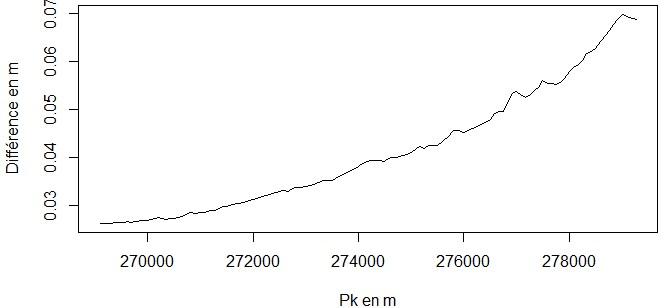
\includegraphics[width=.7\linewidth]{Figures/DiffMerArles.jpg}
        \caption{Différence de hauteur d'eau sur le bief Beaucaire-Diffluence pour une limite aval au niveau de la mer ou au niveau de la ville d'Arles. La station de Beaucaire Restitution se situe au PK 269.5 (à gauche) et la ville d'Arles au PK 282.2, soit environ 2 km à l'aval de la diffluence (à droite).}
		\label{fig:DifMerArles}
	\end{figure}			 
	 
	\paragraph{} Afin d'adapter la géométrie des sections à des débits importants, des points supplémentaires ont été ajoutés au modèle pour représenter le lit majeur. L'altitude de ces points est basée sur les données MNT de la base de données topographique (BDT) du Rhône dont les mesures ont été réalisées en 2010 dans le cadre du Plan Rhône. Les sections en travers sont prolongées jusqu'aux digues de protection actuelles (figure \ref{fig:Elarg}) qui protègent des débordements au moins jusqu'au niveau de la crue de 2003, soit une crue environ centennale. 
	
	\begin{figure}[h]
	\centering
		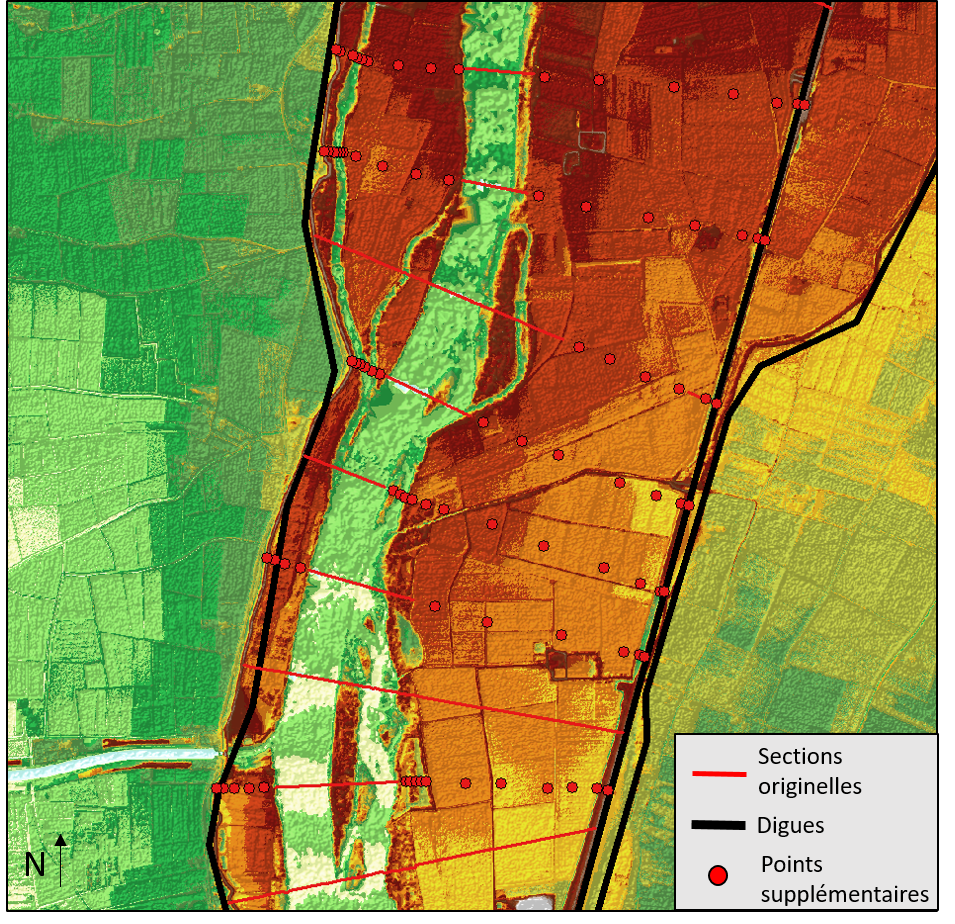
\includegraphics[width=.5\linewidth]{Figures/Elarg.png}
        \caption{Élargissement des sections en travers du modèle jusqu'aux limites du lit majeur (digues). L'altitude des points est basée sur le MNT de la BDT Rhône de 2010 }
		\label{fig:Elarg}
	\end{figure}		
	
	\paragraph{} Afin de se placer dans le contexte historique pré-aménagements CNR, les aménagements présents dans le modèle sont supprimés. Il s'agit de l'usine de Beaucaire, du barrage de Vallabrègues, ainsi que du seuil de Beaucaire. La topologie du modèle suite à ces simplifications est présentée dans la figure \ref{fig:Mageavap} (droite).
	
	\begin{figure}[h]
	\centering
		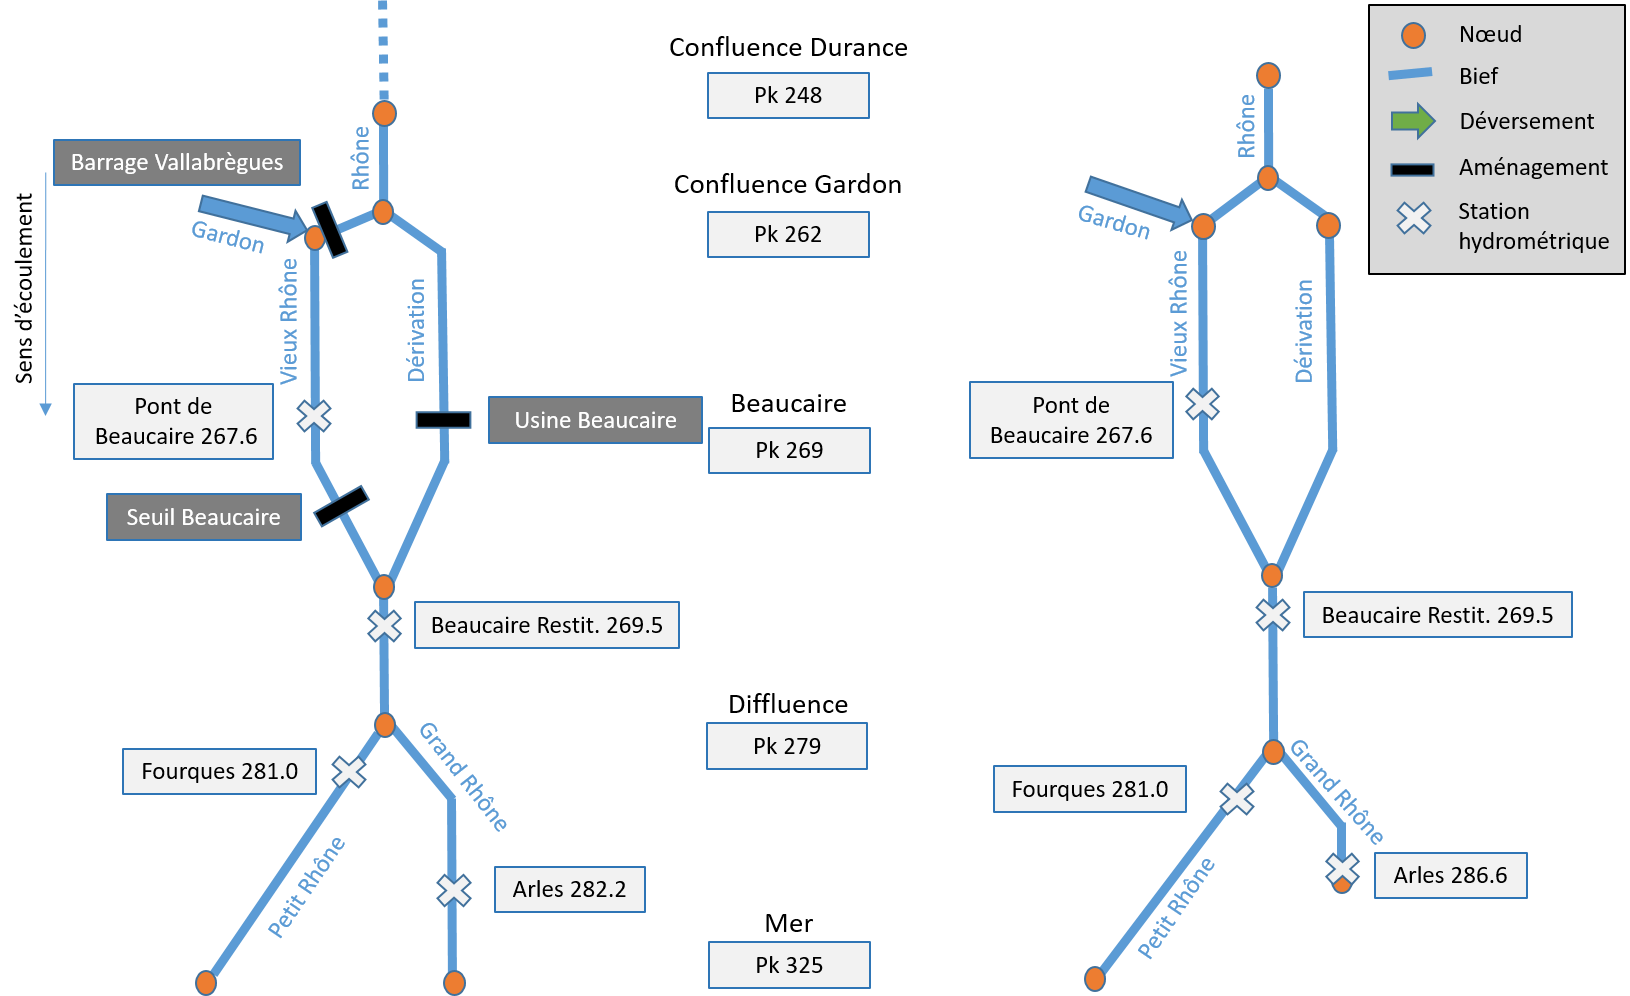
\includegraphics[width=.9\linewidth]{Figures/MAGERh_AvAp.png}
        \caption{Topologie du modèle avant (gauche) et après simplifications (droite).}
		\label{fig:Mageavap}
	\end{figure}		
			
	\subsection{Sensibilité du modèle}
		
	\paragraph{} La sensibilité du modèle hydraulique à plusieurs scénarios a été testée afin de connaitre l'impact de la prise en compte (ou de la non-prise en compte) précise de ces scénarios dans le cadre de reconstitutions historiques. La référence de ces tests est le modèle présenté à la section précédente, pour lequel les aménagements hydroélectriques ont été supprimés, les sections en travers ont été élargies jusqu'aux limites du lit majeur, et la limite aval du Grand Rhône a été fixée à Arles. Les simulations suivantes représentant diverses hypothèses seront donc comparées à cette simulation de référence. La différence de hauteur au niveau de la station de Pont de Beaucaire sera notamment étudiée.
	
	\paragraph{} On cherche à reproduire ici une crue centennale similaire à la crue de Décembre 2003 au cours de laquelle le débit à Beaucaire était d'environ 11 500 m\textsuperscript{3}/s. La condition limite amont (nœud à l'aval de la confluence avec la Durance) est représentée par un hydrogramme permanent de 10 500 m\textsuperscript{3}/s. La confluence du Gardon est représentée par un apport latéral constant de 1000 m\textsuperscript{3}/s. La limite aval pour le bief du Petit Rhône est représentée par un niveau de la Mer Méditerranée de 0.136 m. La limite aval du Grand Rhône est représentée par un limnigramme constant à 7.03 m, soit la hauteur maximale enregistrée lors de la crue de 2003. Le calage des coefficients de frottements (Strickler) du modèle OSR (REF LAUNAY 2015) est conservé, bien que ces derniers ne soient valable que jusqu'à la crue décennale. Le temps de simulation est de 10 heures afin d'aboutir à une convergence satisfaisante, et le pas de temps de simulation est de 60 secondes. Les résultats de cette section sont des résultats partiels qui ont pour unique but d'identifier les points clés de la modélisation d'événements historiques, et notamment d'identifier les simplifications possibles du modèle qui ne dégradent pas grandement la qualité des estimations.
	
	\begin{figure}[h]
		\centering
		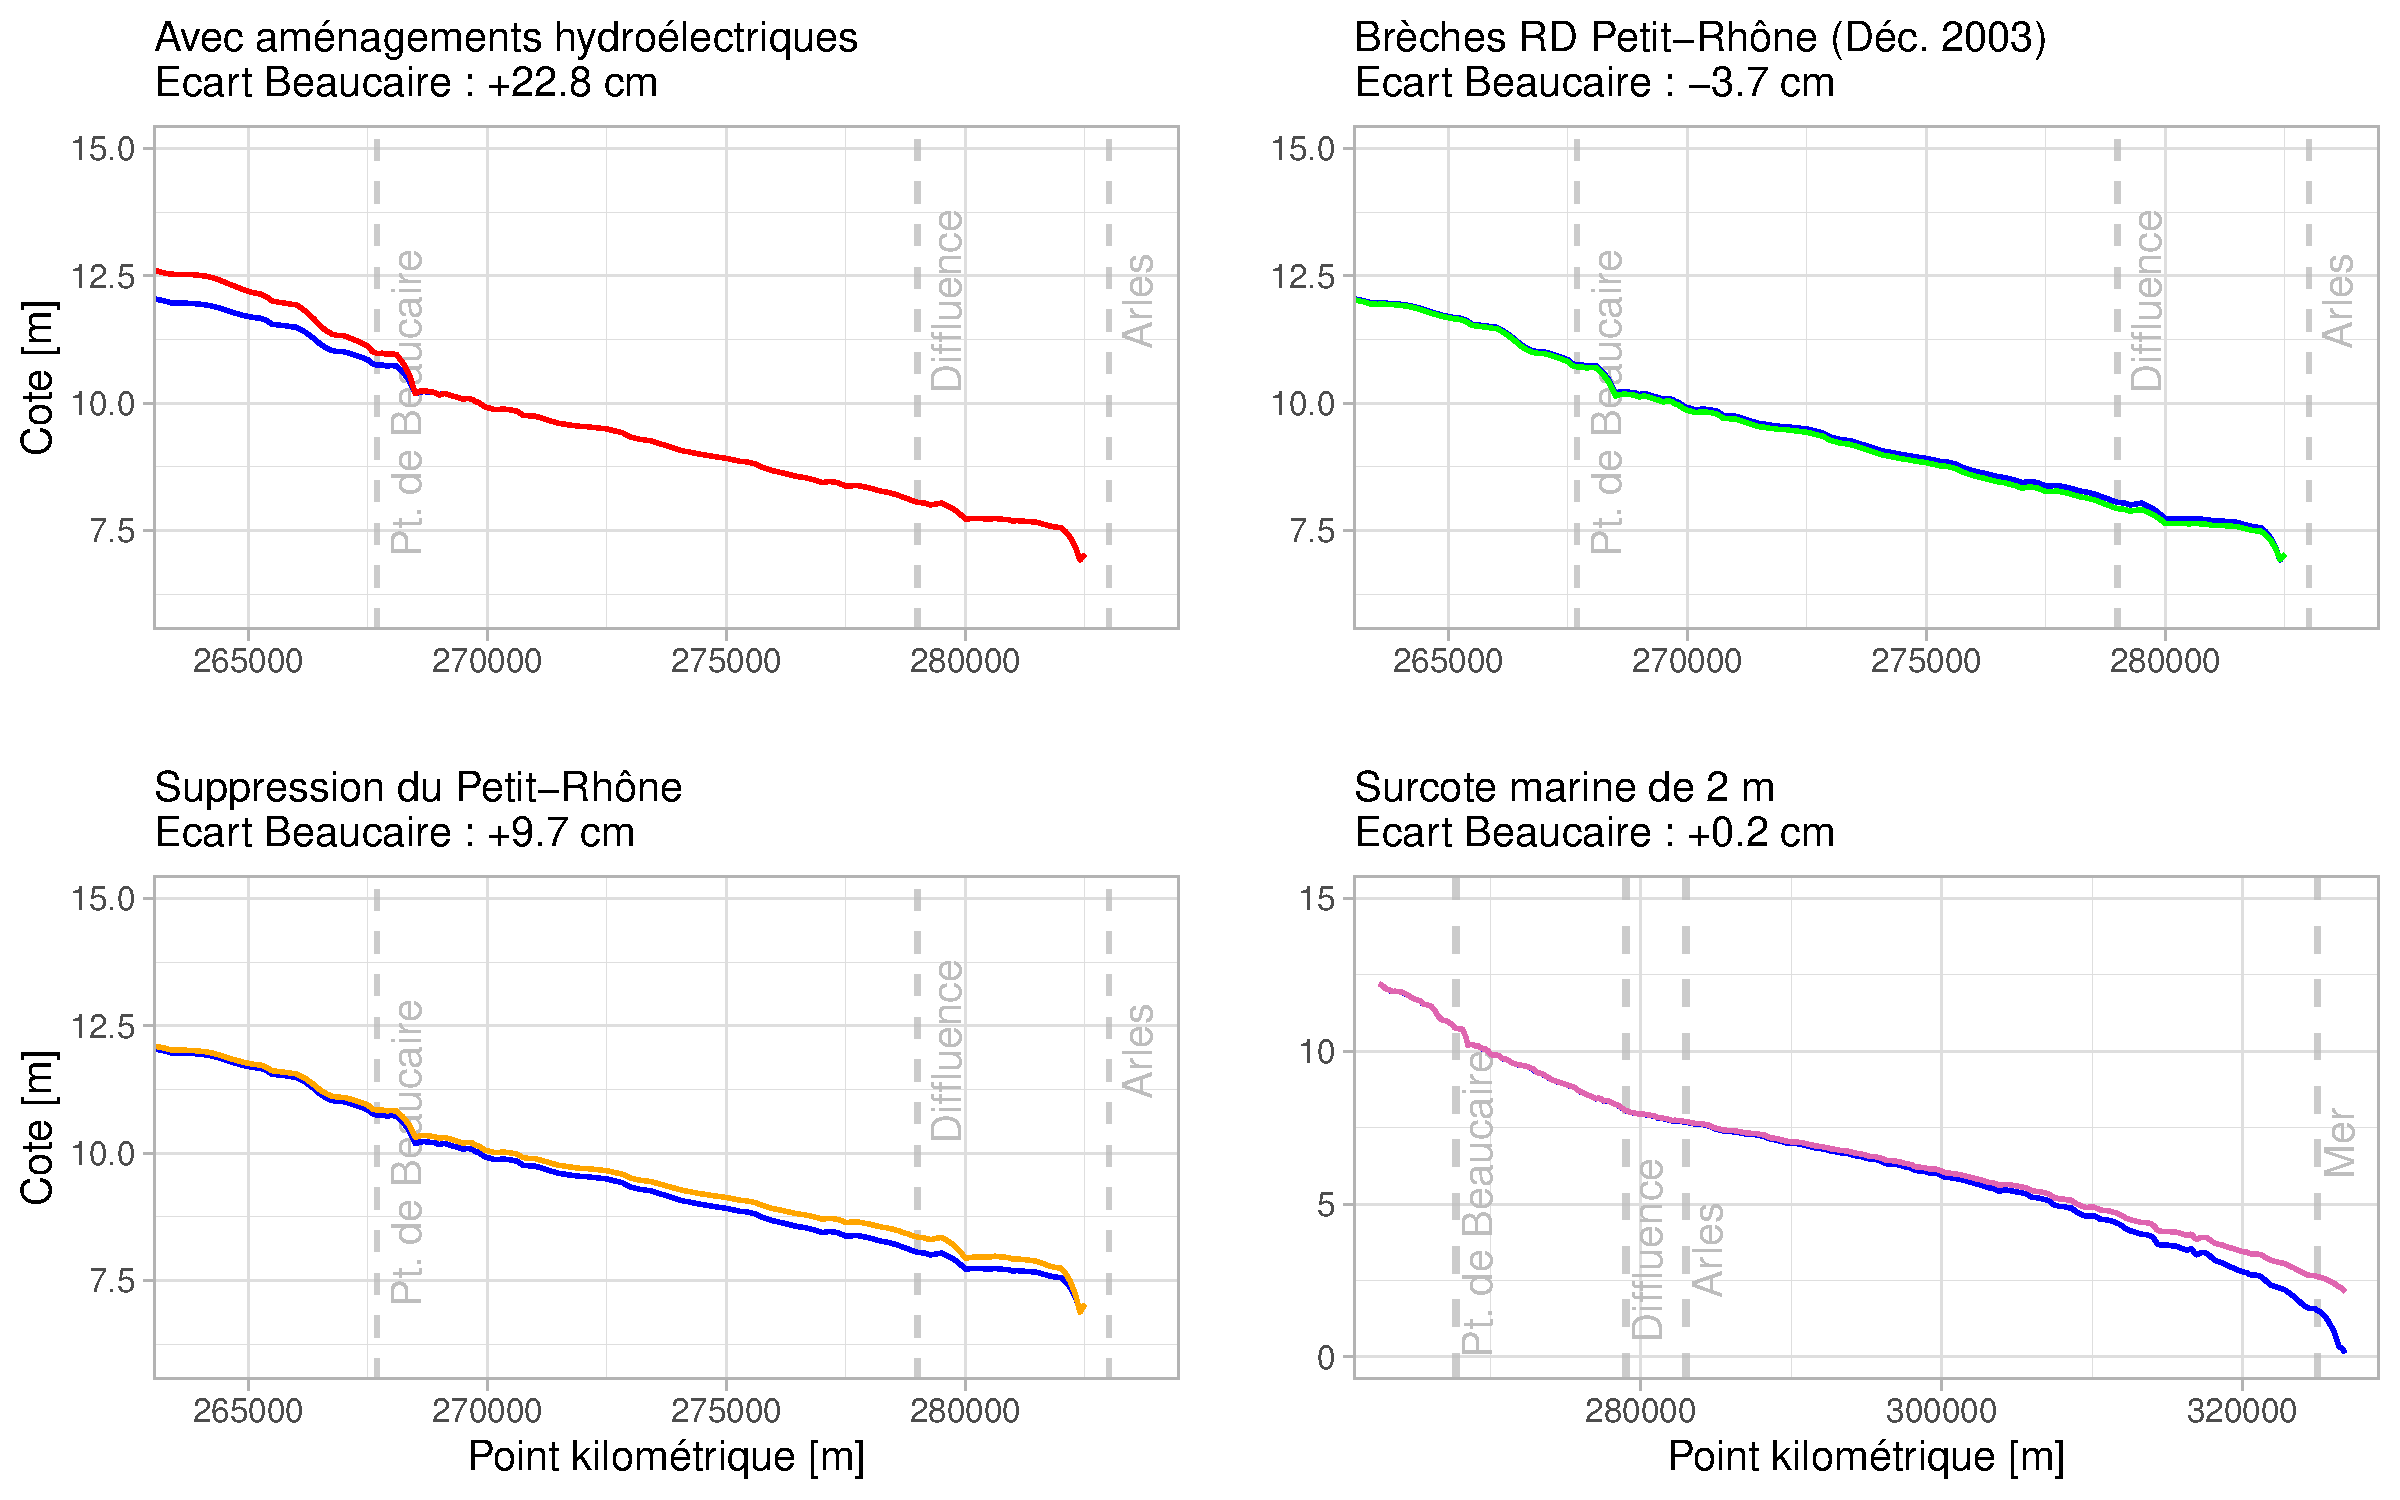
\includegraphics[width=\linewidth]{Figures/4cases.pdf}
        \caption{Vieux Rhône, Rhône, Grand-Rhône/Petit-Rhône}
		\label{fig:Sensib4}
	\end{figure}		
			
	
	\subsubsection{Sensibilité aux aménagements hydroélectriques}
	
		\paragraph{} Les aménagements hydroélectriques CNR ont été construits entre 1967 et 1970 et ont une influence sur la ligne d'eau à Beaucaire. Ces aménagements sont représentés dans le modèle OSR originel (REF DUGUE 2014) sous forme de lois ouvrage de nature différentes, ces lois seront reprises ici. Par exemple, le barrage de Vallabrègues est représenté par une loi de type seuil/déversoir avec une cote de déversement de 16.63 m, une largeur déversante de 176 m, et un coefficient de débit de 0.4. La vanne de fond est représentée par un orifice rectangulaire dont la cote de déversement correspond à un niveau de 2.03 m, la cote de mise en charge à un niveau de 6.1 m, et la cote de mise en charge maximale à un niveau de 16.6 m. L'usine hydroélectrique et le seuil de Beaucaire sont également représentés dans le modèle (figure \ref{fig:Mageavap}). La suppression des aménagements hydroélectriques dans le modèle semble avoir un impact important sur la ligne d'eau à l'amont du bief Beaucaire-Diffluence, avec une réduction de 22.8 cm de la hauteur d'eau à Pont de Beaucaire (figure \ref{fig:Sensib4}). Néanmoins, le modèle de "référence" n'est absolument pas représentatif des conditions d'écoulement pré-aménagements CNR (avant 1967) étant donné que la géométrie des sections provient de mesures réalisées en 2010. Bien que le Rhône au droit de Beaucaire était historiquement séparé en deux chenaux par des digues, même avant la construction des aménagements CNR (REF CARTE 1950), il faut noter que ces deux chenaux communiquaient à haut débit, ce qui n'est pas le cas ici. 
	
	\subsubsection{Sensibilité à la suppression du Petit-Rhône} 
	
	\paragraph{} La morphologie du Petit-Rhône a profondément évolué au cours des derniers siècles (figure \ref{fig:Embouch}), comme souligné par REF PICHARD 2014 et Raccasi \citet{raccasi_mutations_2008}. De plus, la part de débit correspondant au Petit-Rhône part rapport à celle du Rhône total a probablement évolué au gré de ses évolutions morphologiques. Ces changements rendent complexe la reconstitution de la morphologie historique du Petit-Rhône. Afin de s'affranchir de ces reconstitutions, la solution la plus simple et la plus radicale est la suppression du Petit-Rhône du modèle hydraulique, la totalité des débits transitant alors par le bief du Grand-Rhône. On constate sur la figure \ref{fig:Sensib4} que cela a pour conséquence une augmentation de la hauteur d'eau sur l'ensemble du linéaire modélisé. L'augmentation est évidemment maximale sur le bief Diffluence-Arles, et s'élève à 9.7 cm à Pont de Beaucaire. Cet impact sur la ligne d'eau à Pont de Beaucaire est relativement faible. Il correspond à un écart en débit d'environ 300 m\textsuperscript{3}/s, soit une augmentation d'environ 2\% (d'après les courbes de tarage déterminées à Pont de Beaucaire au chapitre 3 REF). La suppression du Petit-Rhône ayant un impact limité sur la hauteur d'eau à Beaucaire, il semble que la solution la plus raisonnable soit de conserver le Petit-Rhône dans le modèle sous sa forme moderne. On suppose donc que les changements morphologique du Petit-Rhône ont un impact très limité sur la hauteur d'eau à Beaucaire.
	
	\subsubsection{Sensibilité aux ruptures de digues}
	
	\paragraph{} De nombreuses crues ont provoqué des ruptures de digues dans l'histoire du bas-Rhône \citep{pichard_sept_2014}, notamment en 2003 \cite{medd_debit_2005}. La reconstitution de ces ruptures de digues pour les crues historiques est complexe, notamment en ce qui concerne la largeur et la profondeur de la rupture. L'importance de la prise en compte des ruptures de digues dans le modèle est étudiée en reproduisant les dommages observés en 2003 sur le Petit-Rhône. Plusieurs brèches dans les digues sont survenues pendant cet événement et sont résumées dans la figure \ref{fig:Breches2003} tirée de l'étude du \citet{symadrem_programme_2012}. Dans cette étude, l'impact des brèches des trémies du Mas Tessier et des Ségonnaux (bief Beaucaire-Diffluence) sur la ligne d'eau a Beaucaire a été jugé faible. Seules les brèches du Petit-Rhône (Mas d'Argence et Claire Farine) seront donc reproduites ici. Ces deux brèches sont représentées par des déversements vers l'extérieur du modèle dont la profondeur et la largeur des brèches proviennent des informations présentées en figure \ref{fig:Breches2003}. Les brèches sont supposées actives tout au long de la simulation, leur dynamique n'ayant pas de sens dans le cadre d'une simulation en régime permanent. On constate sur la figure \ref{fig:Sensib4} que l'impact des brèches du Petit-Rhône est faible, et qu'il est maximal a proximité de la diffluence. La hauteur d'eau à Pont de Beaucaire est 3.7 cm plus basse que pour la simulation de référence. Cet écart très faible indique que la considération de ce type de brèche a un impact très limité à Beaucaire. Des conclusions différentes auraient pu être tirées dans le cas de brèches à l'aval ou à l'amont immédiat de Beaucaire qui ont fréquemment été observées par le passé \citep{pichard_sept_2014}. De plus, ce résultat n'est pas représentatif de l'impact des brèches sur la dynamique de la crue, la simulation ayant été réalisée en régime permanent.
	
	\begin{figure}[h]
		\centering
		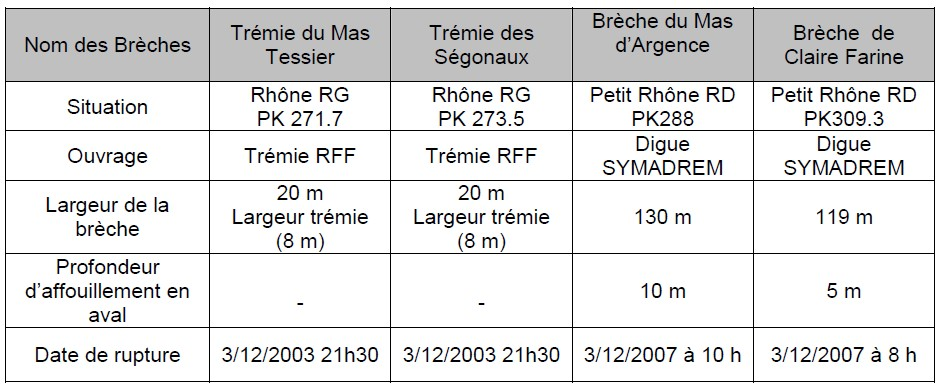
\includegraphics[width=.7\linewidth]{Figures/Breches2003.jpg}
        \caption{Caractéristiques des brèches dans les digues lors de la crue de Décembre 2003, tiré de l'étude du \citet{symadrem_programme_2012}.}
		\label{fig:Breches2003}
	\end{figure}		
	
	\subsubsection{Sensibilité aux surcotes marines}	
	
	\paragraph{} Les surcotes marines sont fréquentes en Méditerranée lors de conditions météorologiques telles que les tempêtes ou les fortes dépressions. Dans de nombreux témoignages historiques, des crues du bas-Rhône sont associées à des tempêtes maritimes \citet{pichard_sept_2014}. Ces augmentations périodiques du niveau de la mer peuvent avoir une influence sur les niveaux d'eau du Rhône. Cet impact est étudié en augmentant artificiellement le niveau de la mer en condition limite aval du modèle pour le bief du Petit-Rhône. La limite aval pour le bief du Grand-Rhône, située à Arles, n'est pas modifiée dans ce scénario. On suppose une surcote marine centennale, estimée à +2 m par KERGADALLAN REF. On constate dans la figure \ref{fig:Sensib4} que l'impact de la surcote est maximal au niveau de la mer et décroit vers l'amont. Il semble important sur le bief du Petit-Rhône, mais la différence de hauteur d'eau à Pont de Beaucaire est proche de zéro. Suite à ce constat, il ne semble pas pertinent de considérer les surcotes marines pour la modélisation des crues historiques à Beaucaire. Cependant, ce scénario suppose que la hauteur d'eau en crue à Arles n'est pas impactée par la surcote marine, ce qui est peu probable.
	
	\paragraph{} Discussion autres sources d'erreur + effet cumulé de tout ça
strickler pas calés, communication beaucaire, autre?
		
	\subsection{Reconstitution de l'hydraulique ancienne}
	
	
	
	\paragraph{Données dispo}
	bathy 1897
	élargissement sections
	carte P\&C 18XX
	
	
		
	\subsection{Limites et incertitude de la modélisation hydraulique des événements historiques}
Incertitude dans le cas de modèles récents +	
	
	manque d'info sur : 
	- topo histo et limites aval (niveau de la mer par ex?) + petit Rhône
	- brèches : longueur, profondeur, à quel moment pendant la crue ? 
	- dynamique de la crue
	- rugosités et occupation du sol historique
	- niveau atteints (laisses de crues imprécises, infos zones impactées mais rarement profondeur)
	
\section{Évolution du temps de propagation des crues}

	\paragraph{} A Beaucaire, l'augmentation du niveau de protection aux inondations semble diminuer le nombre de crues moyennes mais augmenter les conséquences des crues extrêmes à cause d'une concentration des écoulements (section REF). De plus, kes aménagements en lit mineur du Rhône français, débutés dès la seconde moitié du XIX\textsuperscript{ème} siècle, ont eu des conséquences directes sur la géométrie du chenal. Rapidement, la largeur du lit mineur et la ligne d'eau ont été impactés (REFERENCE RETRACTATION CHENAL, OSR?). 
	
	Une conséquence moins triviale mais à une échelle plus large pourrait être la modification de la dynamique d'écoulement des crues sur le continuum fluvial.
	
	 On peut en effet se demander si la transition d'un style fluvial naturel et complexe vers un chenal unique et plus rectiligne n'aurait eu pour conséquence de modifier la vitesse de propagation des événements de crue, mais également d'impacter le laminage des crues le long de la moyenne et basse vallée du Rhône. 
	
	FIGURE CARTE RHÔNE EN TRESSES ETAT MAJOR VS RHÔNE RECTILIGNE
	
	
	 On peut s'attendre alors à une évolution de la synoptique AUTRE MOT des crues, mais également à une diminution de leur temps de propagation. 
	
	\paragraph{Phases d'aménagement}
		premières digues
		girardon
		CNR
		
	\subsection{Sélection de crues océaniques}
	océanique (description pardé)
	non débordant
	visuellement Ok, pas de perturbation de la pointe entre lyon et Bcr
	tableau crues sélect ? ou annexes
	
	\subsection{Résultats}
	boxplot t propag

	\begin{figure}[h]
	\centering
		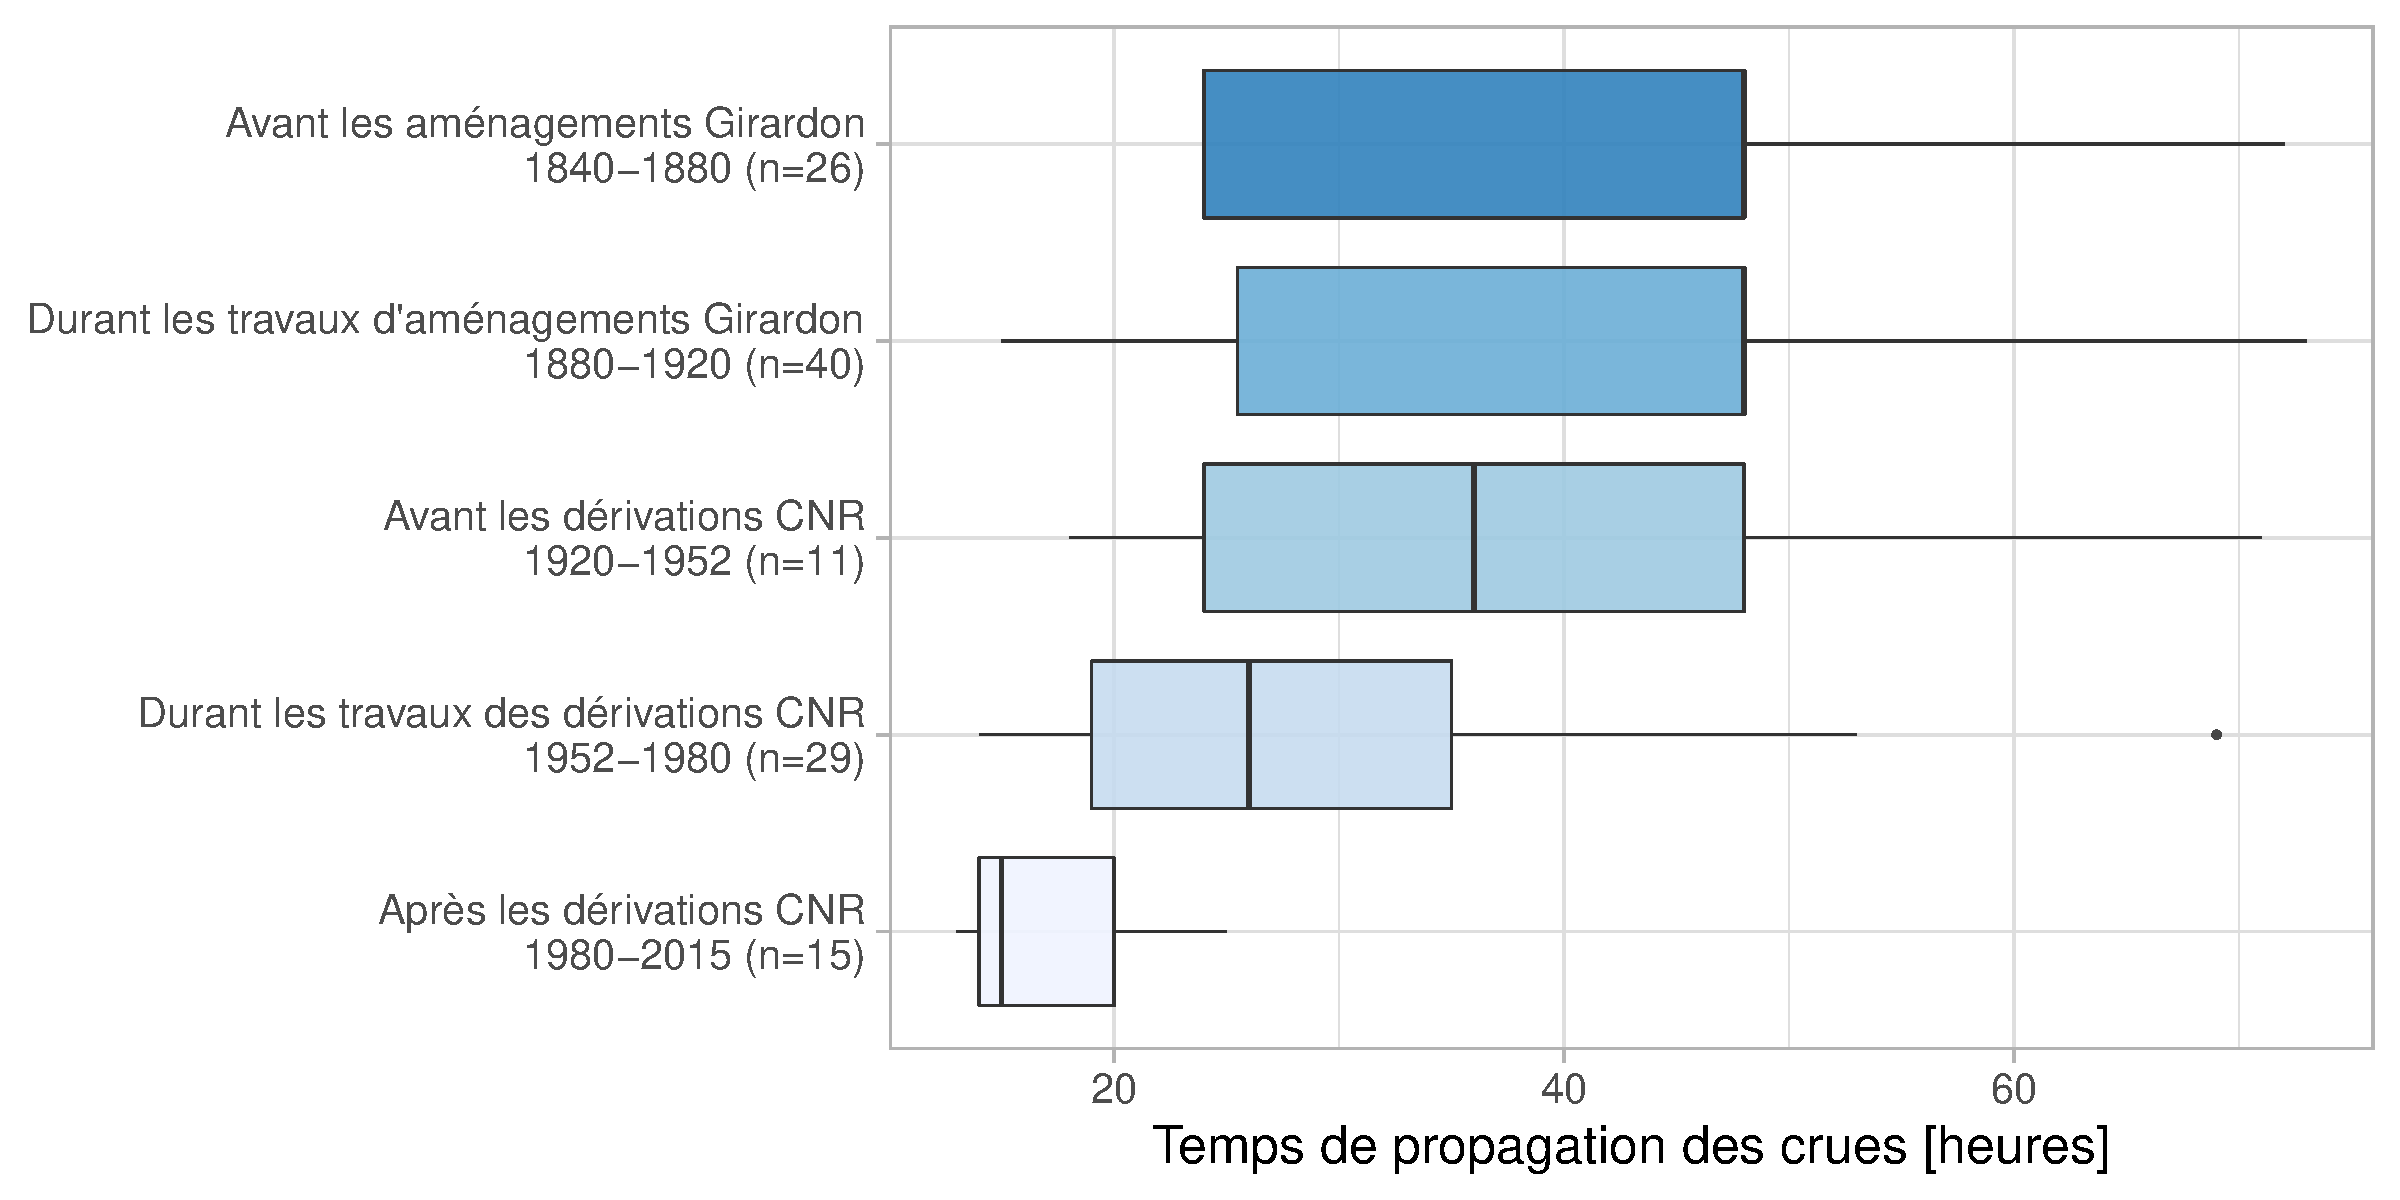
\includegraphics[width=.9\linewidth]{Figures/BoxplotTprop_Fr.pdf}
        \caption{Boites à moustache des temps de propagation de 121 crues océaniques entre Givors et Beaucaire pour 5 périodes d'aménagements en lit mineur (1840-2015).}
		\label{fig:BoxplotPropag}
	\end{figure}	
	
	comparaison référence MAGE
	discussion CF EGR + concomitance + article hossein

OSR
Des limnigrammes du moyen et bas Rhône, antérieurs aux aménagements
Girardon et à ceux de la Compagnie Nationale
du Rhône (CNR), ont été récoltés dans
diverses archives afin de mettre en évidence
d’éventuels effets de ces travaux
sur la dynamique des crues. Ils viennent
s’ajouter à une chronique exceptionnellement
ancienne mesurée à Beaucaire et
débutant en 1816. L’analyse conduite s’est
ainsi limitée au linéaire fluvial entre Lyon
et Beaucaire, considérant que les aménagements
à l’amont de Lyon n’ont eu que
peu d’influence sur la dynamique des
crues du fait de leur forme différente et
de leur moindre présence.
Ont été ainsi compilés les temps de transfert,
entre Lyon et Beaucaire, des crues
d’origine océanique et de périodes de
retour entre 2 et 20 ans (événements
non ou peu débordants). Ces événements
océaniques proviennent de l’amont de
Lyon et se propagent jusqu’à la mer. Lors
de ces épisodes, les affluents du fleuve à
l’aval de Lyon n’ont que peu d’influence
sur les crues. L’analyse du déplacement
de l’onde de crue est ainsi facilitée.
Entre 1840 et 2015, le temps de propagation
de 121 événements a été compilé.
Si le temps moyen mis par les ondes
de crue pour parcourir les 250 km qui
séparent Givors et Beaucaire est de 35h
pour l’ensemble de la période, on constate
des variations de cette durée au cours des
deux siècles d’aménagement du corridor
fluvial. La précision des valeurs de temps
de propagation est à relativiser, principalement
pour les périodes anciennes
au cours desquelles les relevés limnimétriques
étaient effectués une ou trois fois
par jour, causant un arrondi important.
Le passage à trois données par jour en
1910, puis à des données horaires à partir
de 1949, permet d’améliorer la précision
de l’estimation du temps de propagation.
On considère ici que la médiane des événements
de chaque période est un indicateur
pertinent.
Le temps de transfert des crues est en
constante diminution depuis le début du
19ème siècle (FIGURE 4.3). En 175 ans, il est
passé en valeur médiane de 48h avant
la construction des casiers Girardon, à
16h après la construction des aménagements
CNR. Les ouvrages Girardon
semblent avoir, dès la fin du 19ème siècle,
amorcé la réduction de ce temps de propagation
des crues. La diminution importante
des temps de propagation des deux
dernières périodes d’étude indique que les
aménagements hydroélectriques ont eu
un impact encore plus important que les
premiers aménagements en lit mineur.
Les conséquences de ces ouvrages sur
la dynamique des crues peuvent être
diverses. La forme moyenne des hydrogrammes
peut avoir été modifiée et le
pic de crue amplifié par une propagation
devenue plus rapide. Mais la concomitance
entre le pic de crue du Rhône
et celui de ses affluents (en retard sur le
fleuve dans la majorité des cas) peut également
avoir été atténuée, causant un pic
de crue plus faible à l’aval. L’étude de la
forme des hydrogrammes à Beaucaire est
envisagée pour mieux caractériser encore
le phénomène et l’interpréter.


\section{Conclusion}

\section{Annexe 1 : Tableau récap des crues C4 de la base}

\section{Annexe 2 : Tableau des temps de propagation des crues océaniques entre Givors et Beaucaire}


\printbibliography
\end{document}